\chapter{Methodology}
\label{chap:methodology}
\lhead{\emph{Methodology}}
% \rhead{\emph{R00145278}}



\section{Introduction}



This chapter provides a comprehensive and detailed explanation of the techniques and procedures adopted during the course of the research. It serves to provide an in-depth account of the methods used in this study, thereby ensuring the research's transparency and reproducibility.

This research aims to enhance the performance of Optical Character Recognition (OCR) systems - specifically Tesseract OCR and Convolutional Recurrent Neural Network (CRNN) models - on images of sensor readings. To accomplish this, a systematic approach is adopted involving an initial global run of the OCR systems on the raw image datasets, followed by the application of specific image pre-processing techniques and subsequent localized OCR applications.

The purpose of these processes is to establish a baseline of OCR performance, then test the hypothesis that image pre-processing can enhance OCR results. The pre-processing, focused on applying colour masks before converting the images to grayscale, aims to increase the clarity of the images, thereby increasing the efficiency of the OCR processes.

This chapter outlines each of these processes in detail, thereby providing a clear roadmap of the research methodology adopted in this study. From the initial assessment of the OCR systems' performance to the implementation of the pre-processing techniques, this chapter serves as a guide to understanding the practical steps taken during this research project.

The subsequent sections provide further detail on the data being used, the OCR systems of focus, the pre-processing techniques applied, and the methods of evaluation. The goal of this chapter is to present a detailed and comprehensive account of the methodology that underpins this research.

---


\section{Data Collection}

The dataset used in this research is derived from actual industrial meters and not from simulated data. It was supplied as a collection of image files distributed across eight distinct folders. Each folder corresponds to a unique sensor from which readings were taken. These real-world images provide a diversified dataset due to variations in sensor specifications and the conditions under which the readings were captured, underscoring their importance and value for genuine, practical applications.

Upon receiving the data, an initial examination was carried out to ensure the integrity and completeness of the files. The image files were found to be in good condition, readable, and ready for further processing and analysis.

To streamline data management and facilitate the analysis process, a CSV file was compiled. This file serves as an inventory, cataloguing each image file name alongside its corresponding label, thereby establishing an efficient cross-referencing system for the ensuing data analysis phase.

To foster the training of the Convolutional Recurrent Neural Network (CRNN) models, several training databases were established. Each of these databases comprises 500,000 single-digit training images, laying a solid groundwork for the machine learning tasks.


\newpage
\section{Data Analysis}

For each folder, there are three charts that provide an initial statistical data analysis of the images. These charts are as follows:


\begin{enumerate}
    \item \textbf{Montage:} A simple representation of the images in the folder, arranged in a grid format. This provides a visual overview of the images in the folder, thereby facilitating a quick assessment of the data.
    \item \textbf{RGB Histogram:} This chart shows the distribution of pixel intensities for the Red, Green, and Blue channels separately in each image.
          \begin{enumerate}

              \item \textit{Axes:} The X-axis represents the possible pixel intensity values (ranging from 0 to 255 for an 8-bit image), and the Y-axis represents the number of pixels in the image with that intensity value.
              \item \textit{Colour Lines:} The Red line shows the distribution of red pixel intensities, the Green line shows the distribution of green pixel intensities, and the Blue line shows the distribution of blue pixel intensities.
              \item \textit{Interpretation:} Peaks in the graph represent the colours that are most present in the image. For instance, a high peak in the red line around the value 200 would indicate that the image has many pixels with high red intensity, suggesting the image may visually appear reddish.
              \item \textit{Colour Composition:} The overall shape of these colour distributions can provide an idea about the colour composition of the images.
              \item \textit{Utility:} The RGB Histogram aids in understanding the dominant colours in the image, the contrast, and the brightness. Variations in these histograms across the image set might be related to different sensor readings or variations in image capture settings.
          \end{enumerate}
          \newpage
    \item \textbf{Data Analysis:} Eight metrics have been defined to quantify various properties of an image. Each of these metrics provides insight into different aspects of the image, allowing for a detailed analysis and comparison of images. These metrics are as follows:
          \begin{enumerate}

              \item \textbf{Contrast:} The Contrast chart visualizes the degree of local variation in an image, which can be associated with the details or changes in sensor readings.
              \item \textbf{Dissimilarity:} Dissimilarity, like contrast, measures local variations, offering additional information about changes in the image.
              \item \textbf{Homogeneity:} The Homogeneity chart shows the closeness of the distribution of elements in an image to its diagonal, providing insight into the uniformity or variation in sensor readings.
              \item \textbf{Energy:} The Energy chart encapsulates the sum of squared elements in the image, which can suggest patterns or randomness in sensor readings.
              \item \textbf{Correlation:} The Correlation chart illustrates the joint probability occurrence of specific pixel pairs, thereby hinting at the predictability or scatter of sensor readings.
              \item \textbf{Area:} The Area chart, in our context, represents the total area of contours detected in an image, providing information on the complexity of sensor readings.
              \item \textbf{Brightness:} The Brightness chart displays the average lightness or darkness of each image, which might be influenced by different environmental conditions or sensor settings.
              \item \textbf{Standard Deviation:} The Standard Deviation chart shows the variability in pixel intensities within each image, helping infer the contrast, detail, and complexity of sensor readings.
          \end{enumerate}


\end{enumerate}

\newpage

% \subsection{Folders}
\subsection{Image Folder A}

There are 167 JPEG files totalling a size of 15.78mb in Image Folder A. The images are of varying dimensions.

\begin{figure}[ht]
    \centering
    \begin{minipage}[t]{0.25\textwidth}
        \centering
        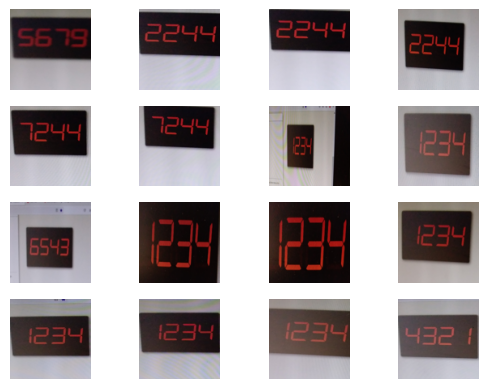
\includegraphics[width=\textwidth]{Figures/EDA_Charts/2/montage.png}
        \caption*{Montage}
    \end{minipage}\hfill
    \begin{minipage}[t]{0.25\textwidth}
        \centering
        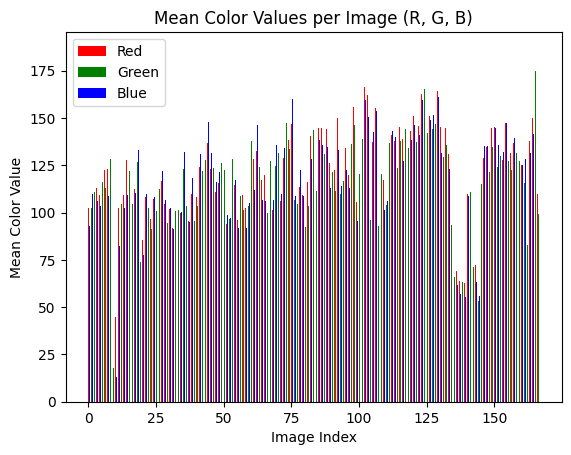
\includegraphics[width=\textwidth]{Figures/EDA_Charts/2/rgb.png}
        \caption*{RGB}
    \end{minipage}\hfill
    \begin{minipage}[t]{0.50\textwidth}
        \centering
        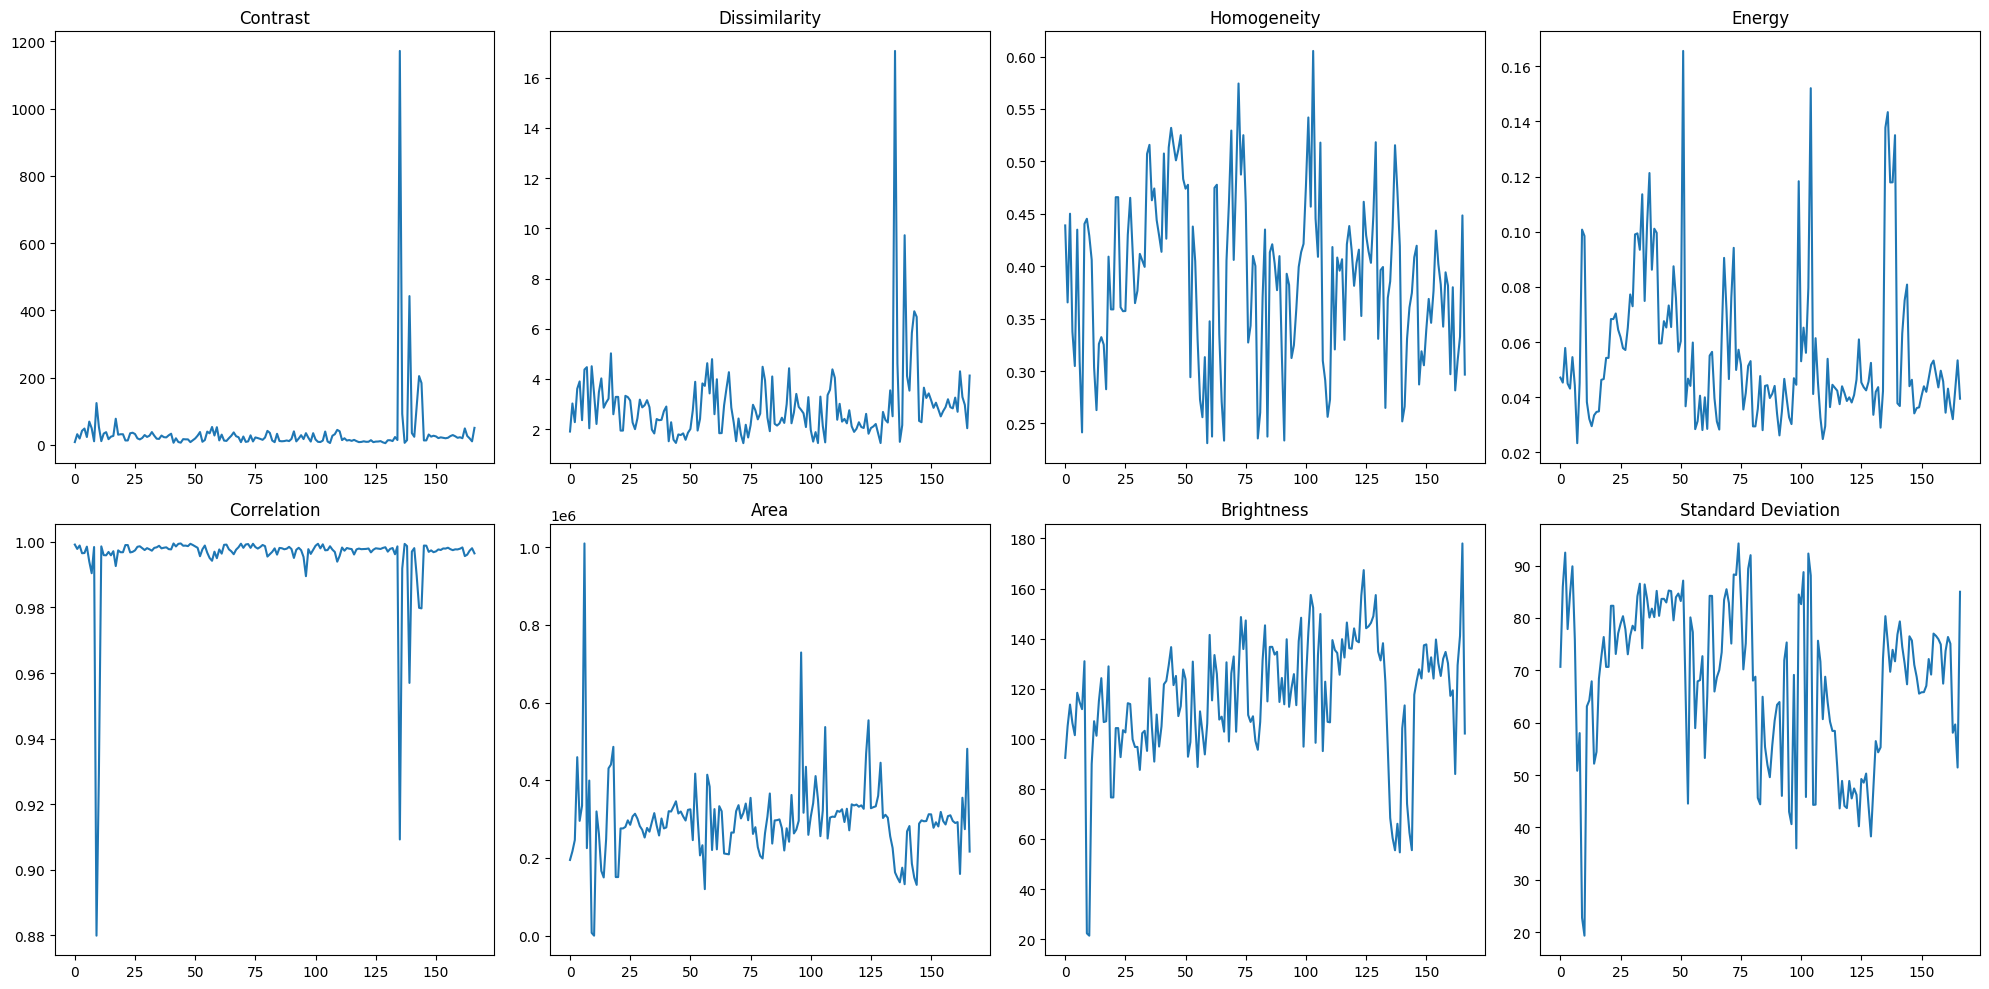
\includegraphics[width=\textwidth]{Figures/EDA_Charts/2/da.png}
        \caption*{Data Analysis}
    \end{minipage}
    \caption{Image Folder A Analysis}
    \label{fig:Image Folder A Analysis}
\end{figure}

\subsection{Image Folder B}

There are 26 JPEG files totalling a size of 77.88mb in Image Folder B. The images are of varying dimensions.

\begin{figure}[ht]
    \centering
    \begin{minipage}[t]{0.25\textwidth}
        \centering
        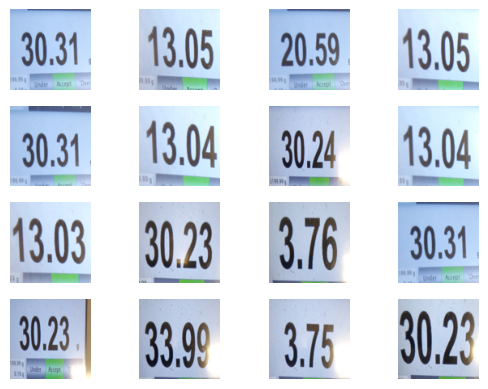
\includegraphics[width=\textwidth]{Figures/EDA_Charts/3/montage.png}
        \caption*{Montage}
    \end{minipage}\hfill
    \begin{minipage}[t]{0.25\textwidth}
        \centering
        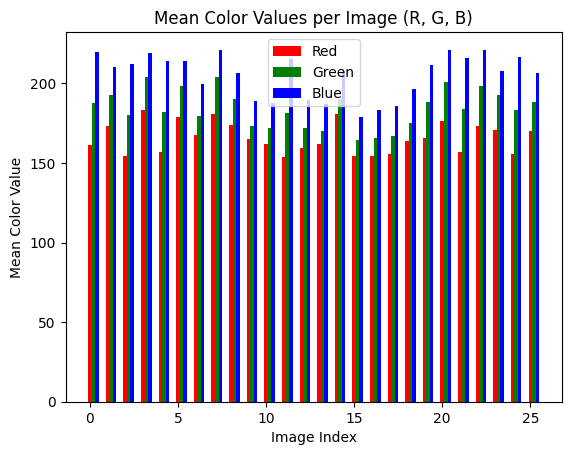
\includegraphics[width=\textwidth]{Figures/EDA_Charts/3/rgb.png}
        \caption*{RGB}
    \end{minipage}\hfill
    \begin{minipage}[t]{0.50\textwidth}
        \centering
        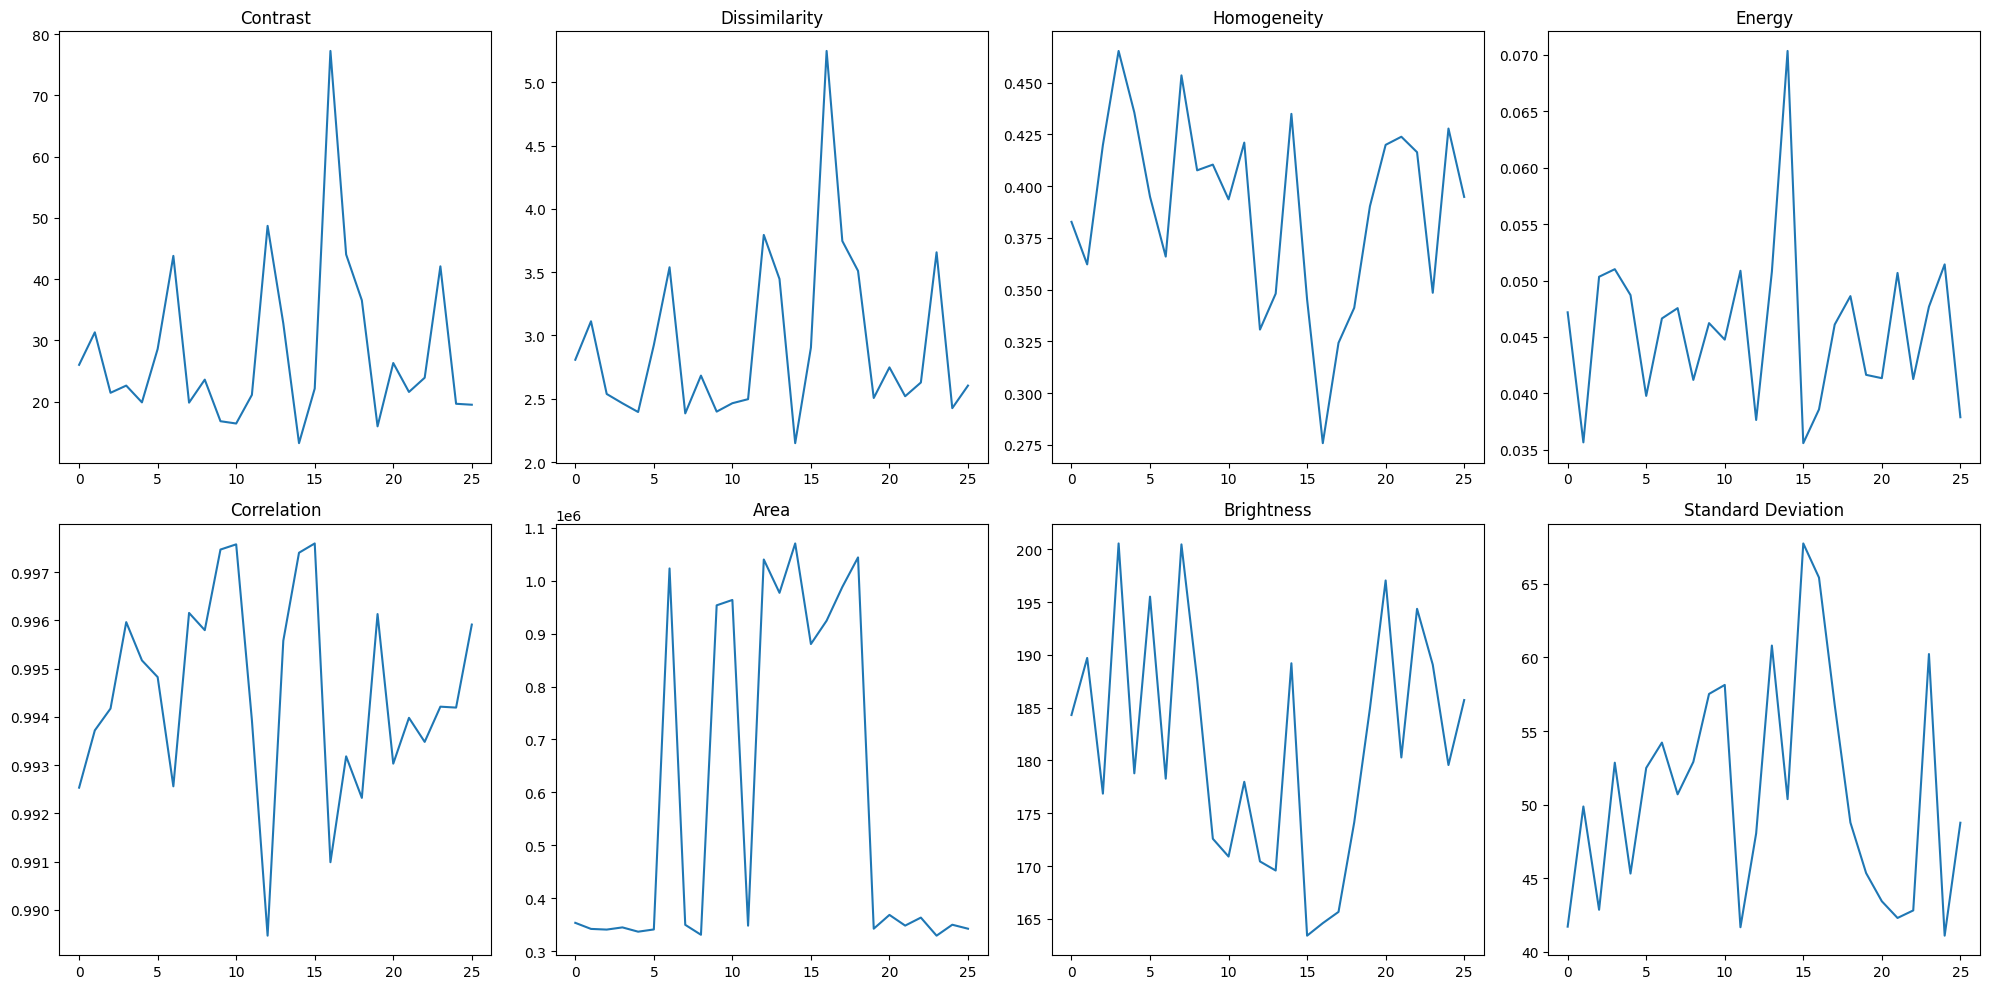
\includegraphics[width=\textwidth]{Figures/EDA_Charts/3/da.png}
        \caption*{Data Analysis}
    \end{minipage}
    \caption{Image Folder B Analysis}
    \label{fig:Image Folder B Analysis}
\end{figure}

\newpage

\subsection{Image Folder C}

There are 10 JPEG files totalling a size of 4.52mb in Image Folder C. The images are of varying dimensions.

\begin{figure}[ht]
    \centering
    \begin{minipage}[t]{0.25\textwidth}
        \centering
        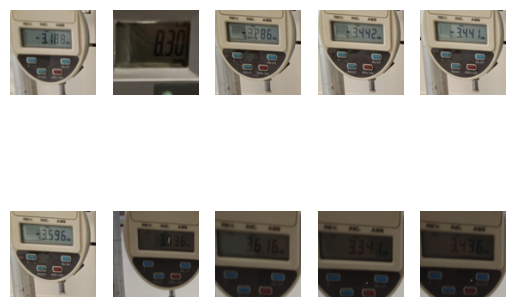
\includegraphics[width=\textwidth]{Figures/EDA_Charts/4/montage.png}
        \caption*{Montage}
    \end{minipage}\hfill
    \begin{minipage}[t]{0.25\textwidth}
        \centering
        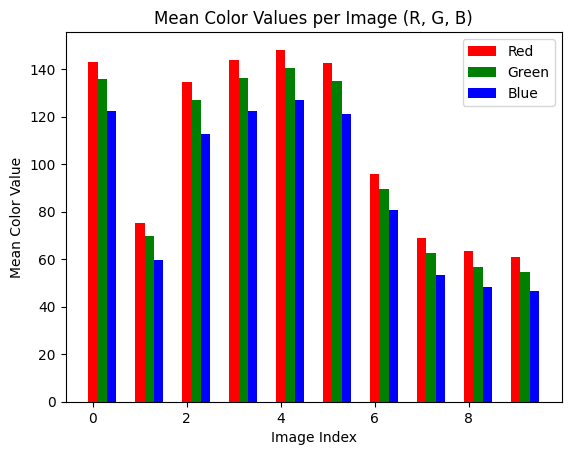
\includegraphics[width=\textwidth]{Figures/EDA_Charts/4/rgb.png}
        \caption*{RGB}
    \end{minipage}\hfill
    \begin{minipage}[t]{0.50\textwidth}
        \centering
        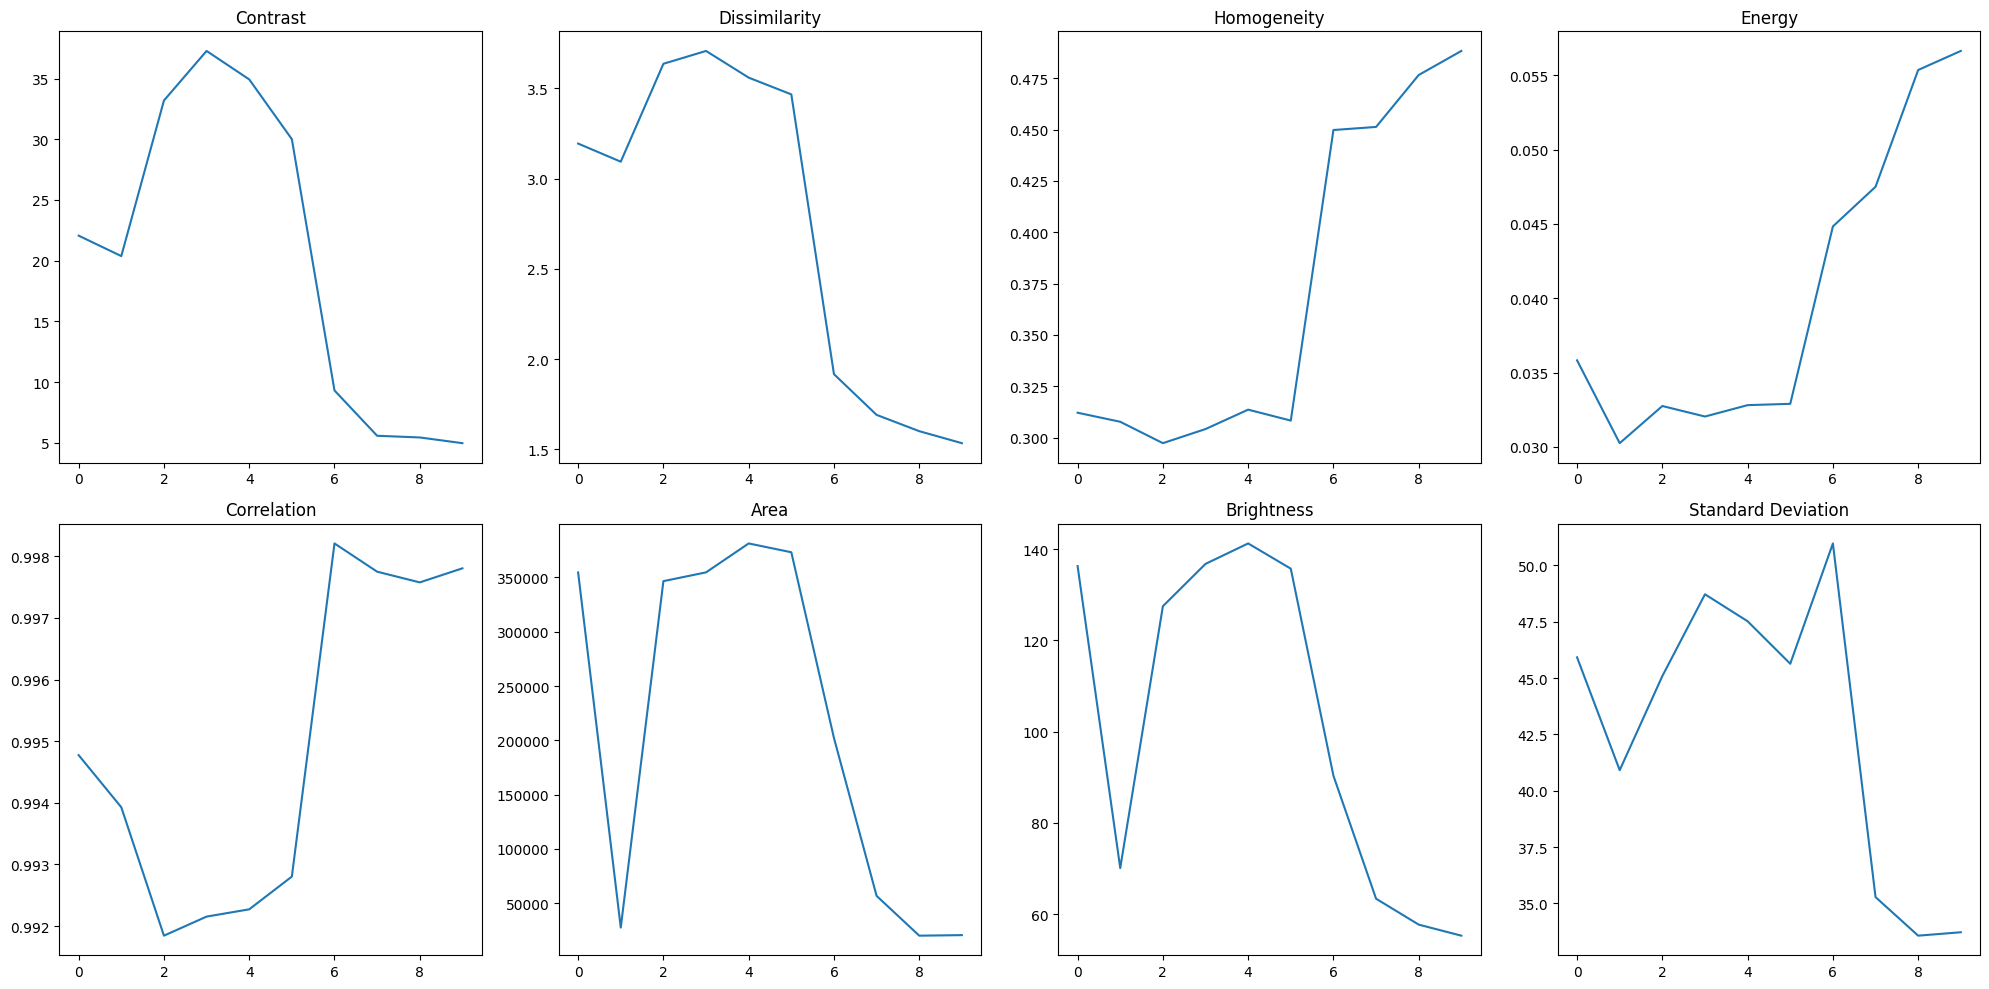
\includegraphics[width=\textwidth]{Figures/EDA_Charts/4/da.png}
        \caption*{Data Analysis}
    \end{minipage}
    \caption{Image Folder C Analysis}
    \label{fig:Image Folder C Analysis}
\end{figure}


\subsection{Image Folder D}

There are 27 JPEG files totalling a size of 6.96mb in Image Folder D. The images are of varying dimensions.

\begin{figure}[ht]
    \centering
    \begin{minipage}[t]{0.25\textwidth}
        \centering
        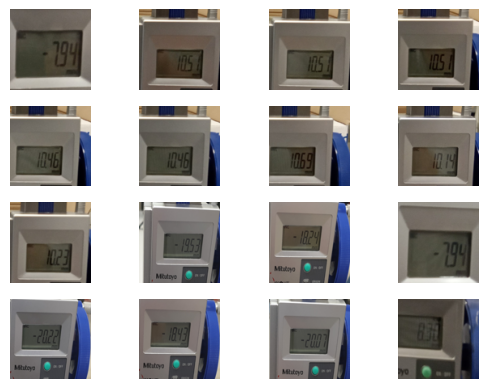
\includegraphics[width=\textwidth]{Figures/EDA_Charts/5/montage.png}
        \caption*{Montage}
    \end{minipage}\hfill
    \begin{minipage}[t]{0.25\textwidth}
        \centering
        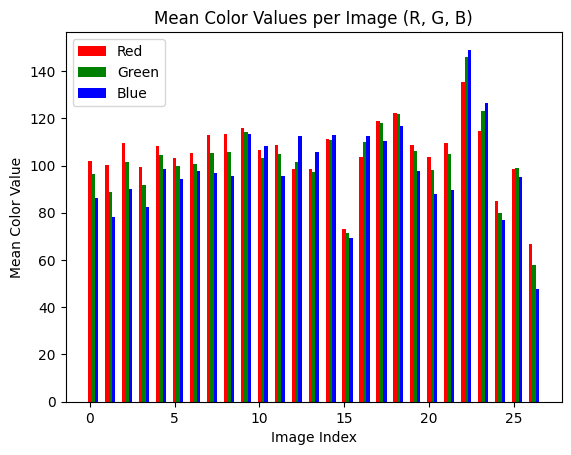
\includegraphics[width=\textwidth]{Figures/EDA_Charts/5/rgb.png}
        \caption*{RGB}
    \end{minipage}\hfill
    \begin{minipage}[t]{0.50\textwidth}
        \centering
        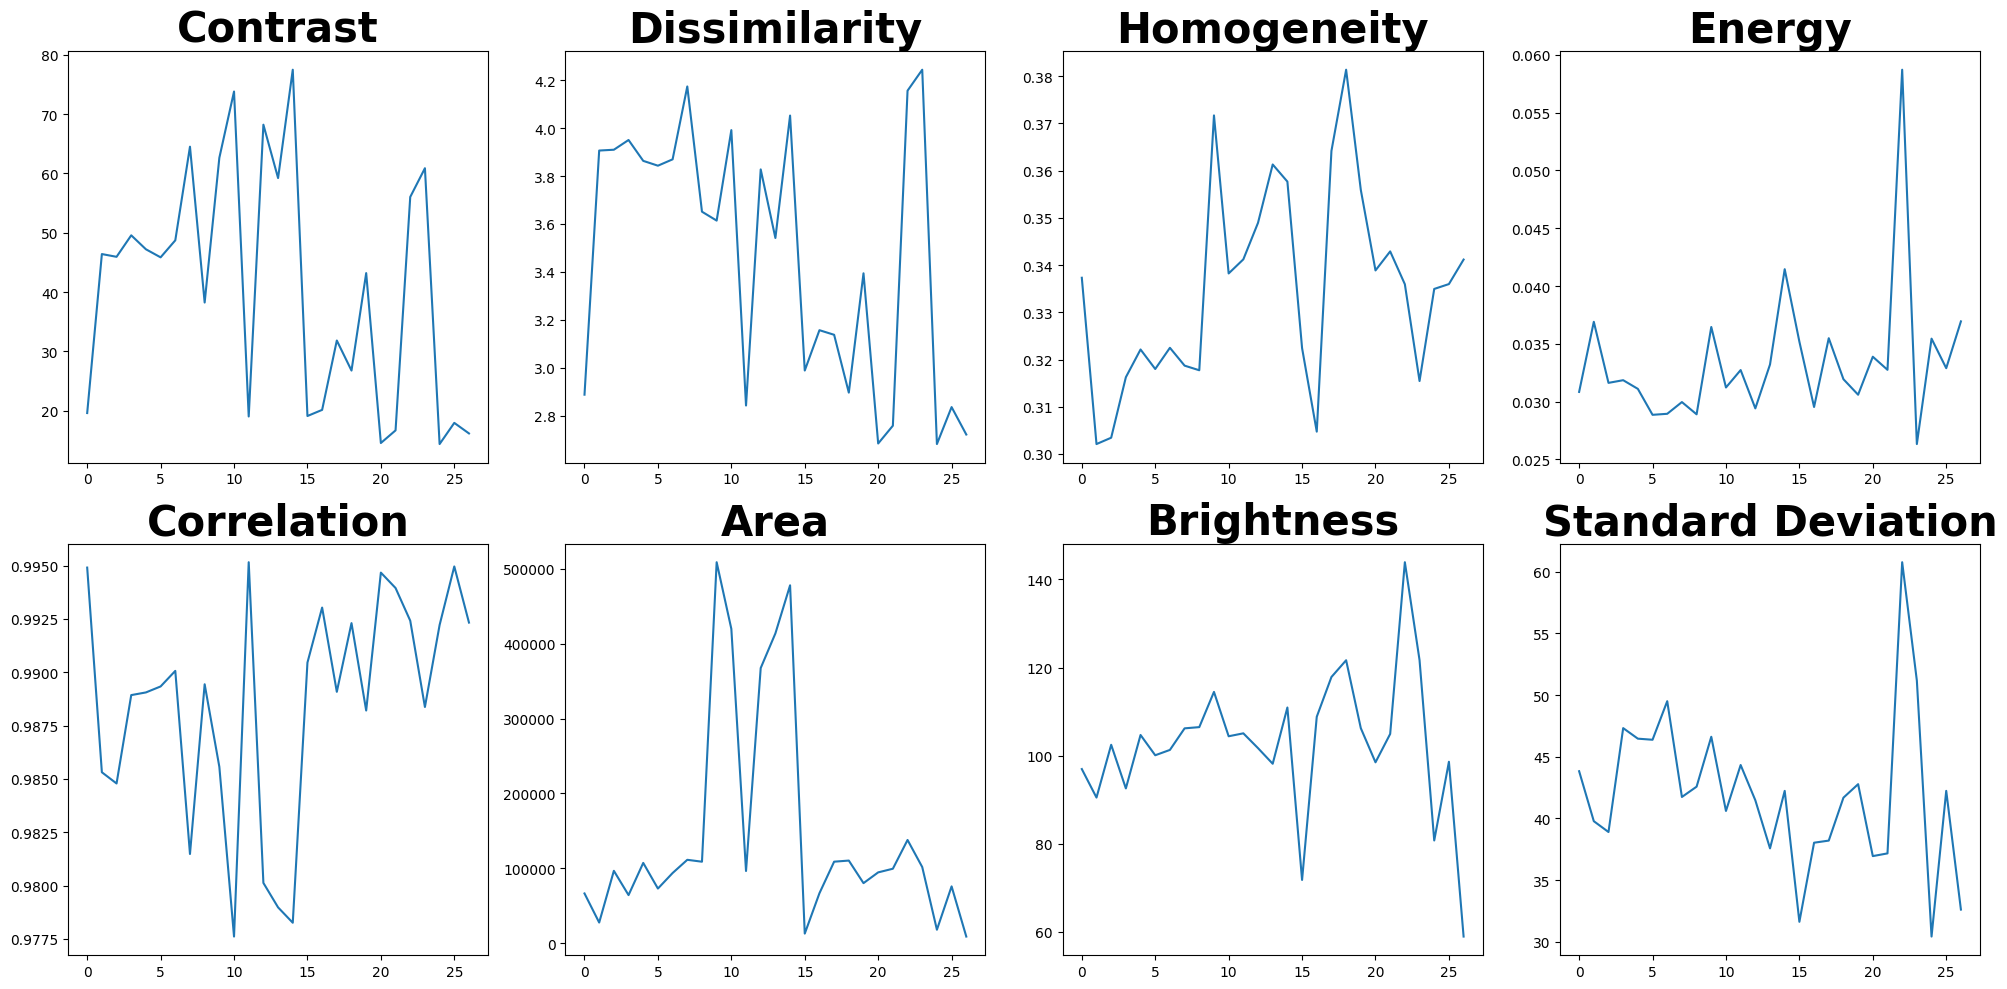
\includegraphics[width=\textwidth]{Figures/EDA_Charts/5/da.png}
        \caption*{Data Analysis}
    \end{minipage}
    \caption{Image Folder D Analysis}
    \label{fig:Image Folder D Analysis}
\end{figure}

\newpage

\subsection{Image Folder E}

There are 10 JPEG files totalling a size of 4.98mb in Image Folder E. The images are of varying dimensions.

\begin{figure}[ht]
    \centering
    \begin{minipage}[t]{0.25\textwidth}
        \centering
        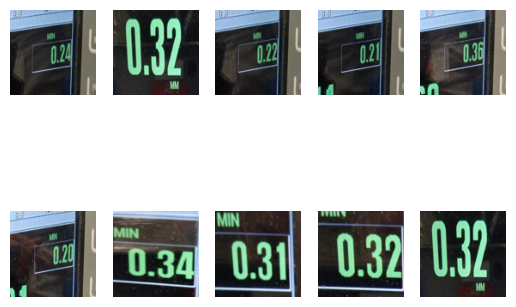
\includegraphics[width=\textwidth]{Figures/EDA_Charts/7/montage.png}
        \caption*{Montage}
    \end{minipage}\hfill
    \begin{minipage}[t]{0.25\textwidth}
        \centering
        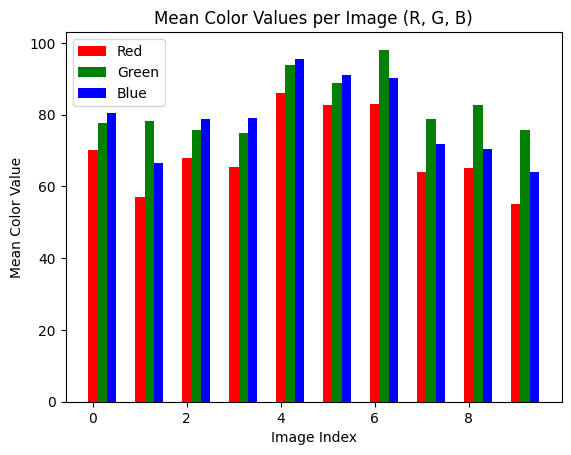
\includegraphics[width=\textwidth]{Figures/EDA_Charts/7/rgb.png}
        \caption*{RGB}
    \end{minipage}\hfill
    \begin{minipage}[t]{0.50\textwidth}
        \centering
        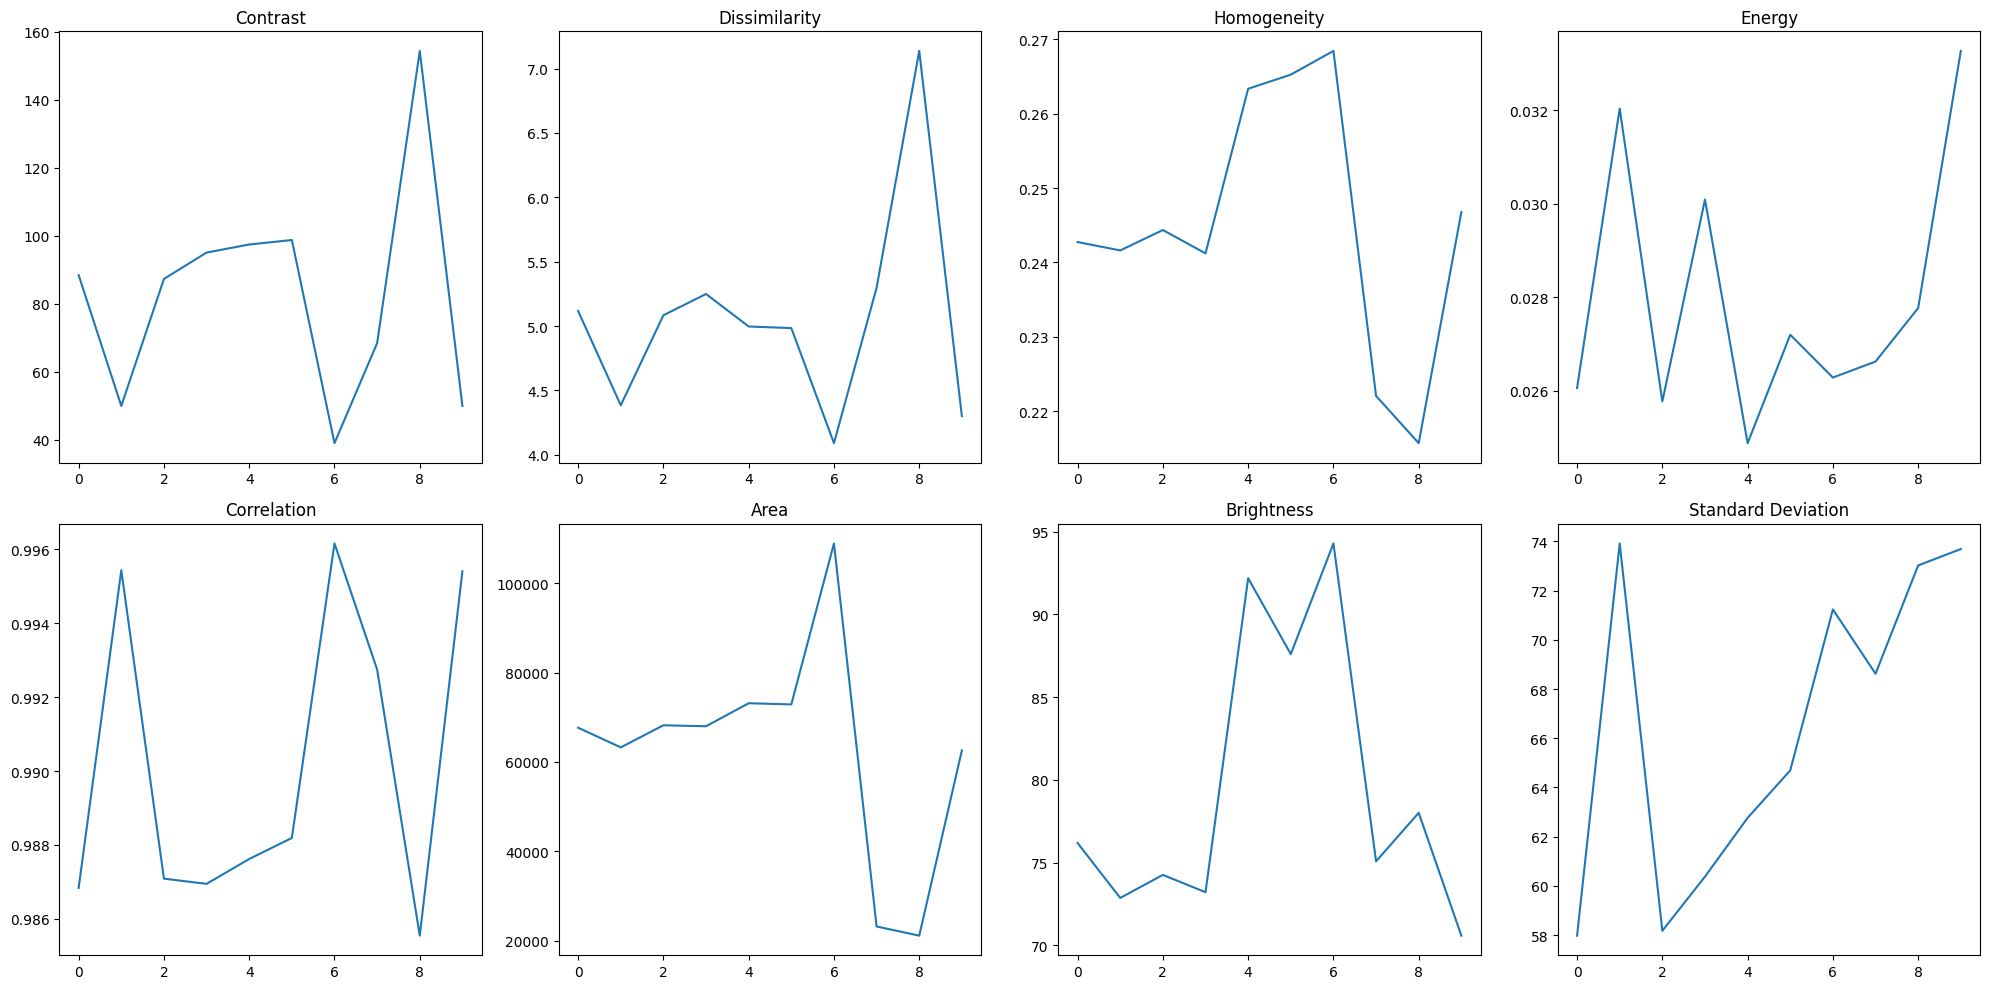
\includegraphics[width=\textwidth]{Figures/EDA_Charts/7/da.png}
        \caption*{Data Analysis}
    \end{minipage}
    \caption{Image Folder E Analysis}
    \label{fig:Image Folder E Analysis}
\end{figure}

\subsection{Image Folder F}

There are 15 JPEG files totalling a size of 5.93mb in Image Folder F. The images are of varying dimensions.

\begin{figure}[ht]
    \centering
    \begin{minipage}[t]{0.25\textwidth}
        \centering
        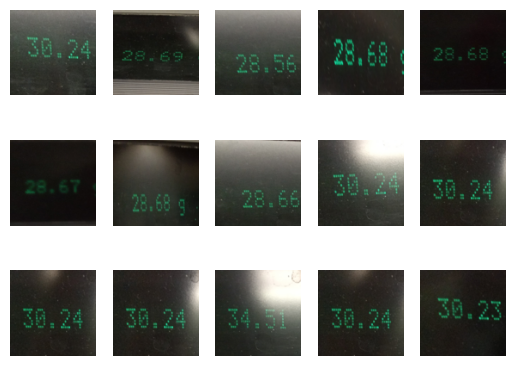
\includegraphics[width=\textwidth]{Figures/EDA_Charts/8/montage.png}
        \caption*{Montage}
    \end{minipage}\hfill
    \begin{minipage}[t]{0.25\textwidth}
        \centering
        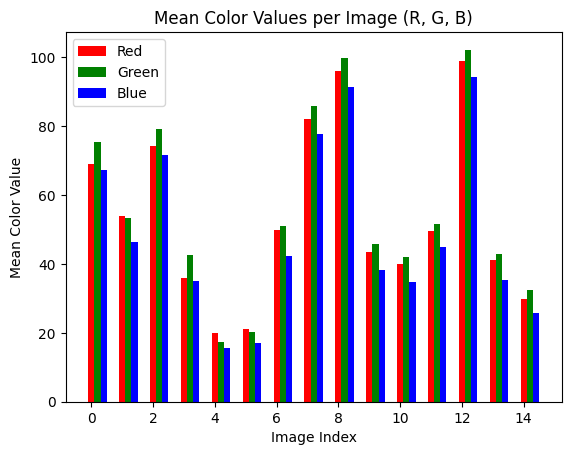
\includegraphics[width=\textwidth]{Figures/EDA_Charts/8/rgb.png}
        \caption*{RGB}
    \end{minipage}\hfill
    \begin{minipage}[t]{0.50\textwidth}
        \centering
        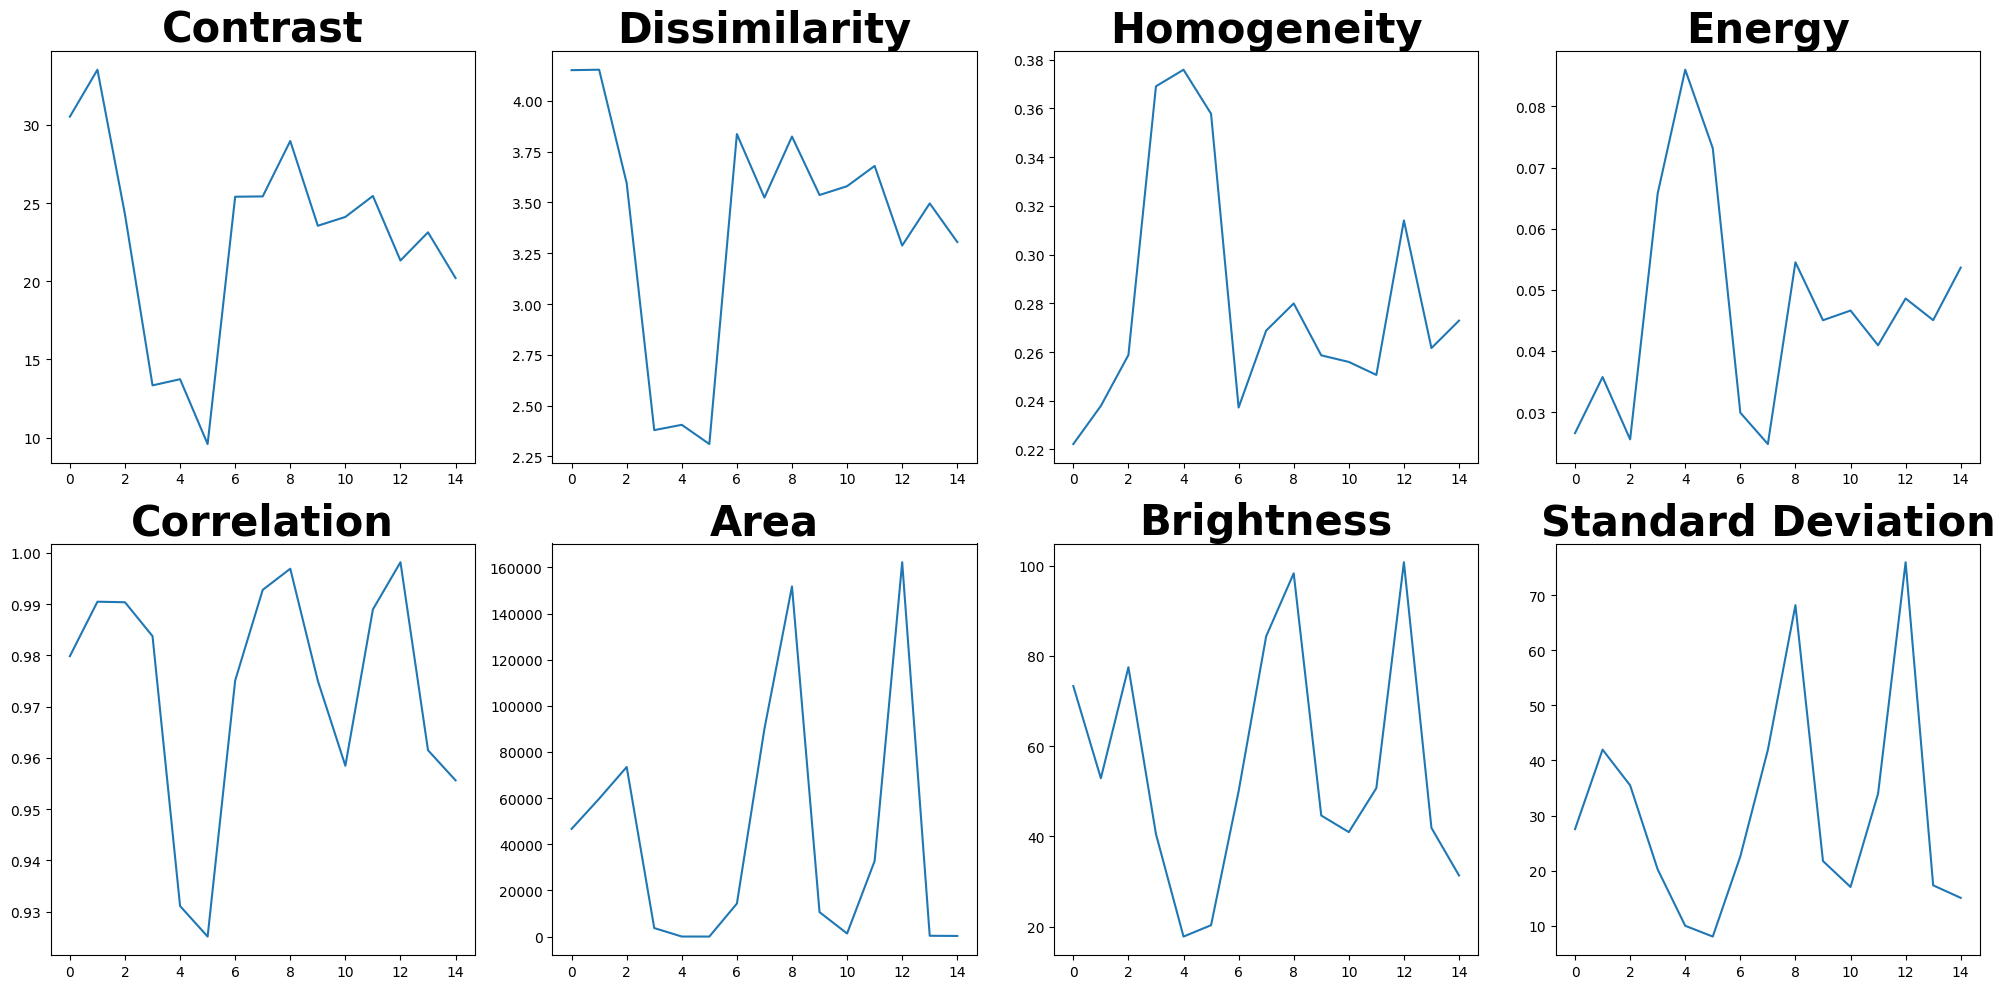
\includegraphics[width=\textwidth]{Figures/EDA_Charts/8/da.png}
        \caption*{Data Analysis}
    \end{minipage}
    \caption{Image Folder F Analysis}
    \label{fig:Image Folder F Analysis}
\end{figure}

\newpage

\subsection{Image Folder G}

There are 12 JPEG files totalling a size of 7.34mb in Image Folder G. The images are of varying dimensions.

\begin{figure}[ht]
    \centering
    \begin{minipage}[t]{0.25\textwidth}
        \centering
        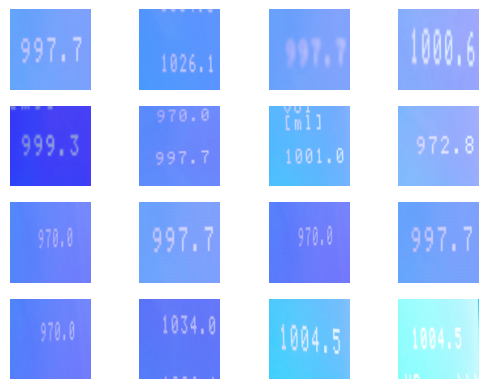
\includegraphics[width=\textwidth]{Figures/EDA_Charts/9/montage.png}
        \caption*{Montage}
    \end{minipage}\hfill
    \begin{minipage}[t]{0.25\textwidth}
        \centering
        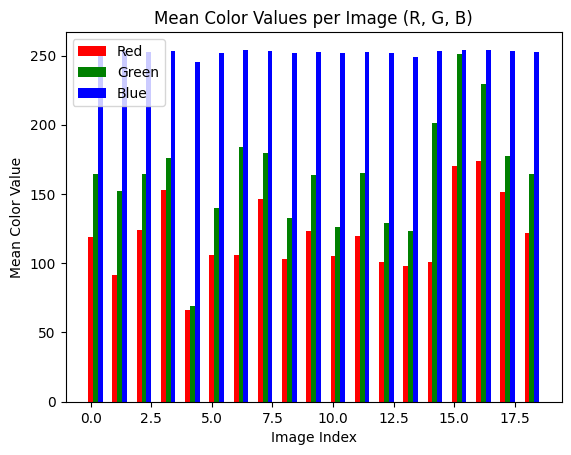
\includegraphics[width=\textwidth]{Figures/EDA_Charts/9/rgb.png}
        \caption*{RGB}
    \end{minipage}\hfill
    \begin{minipage}[t]{0.50\textwidth}
        \centering
        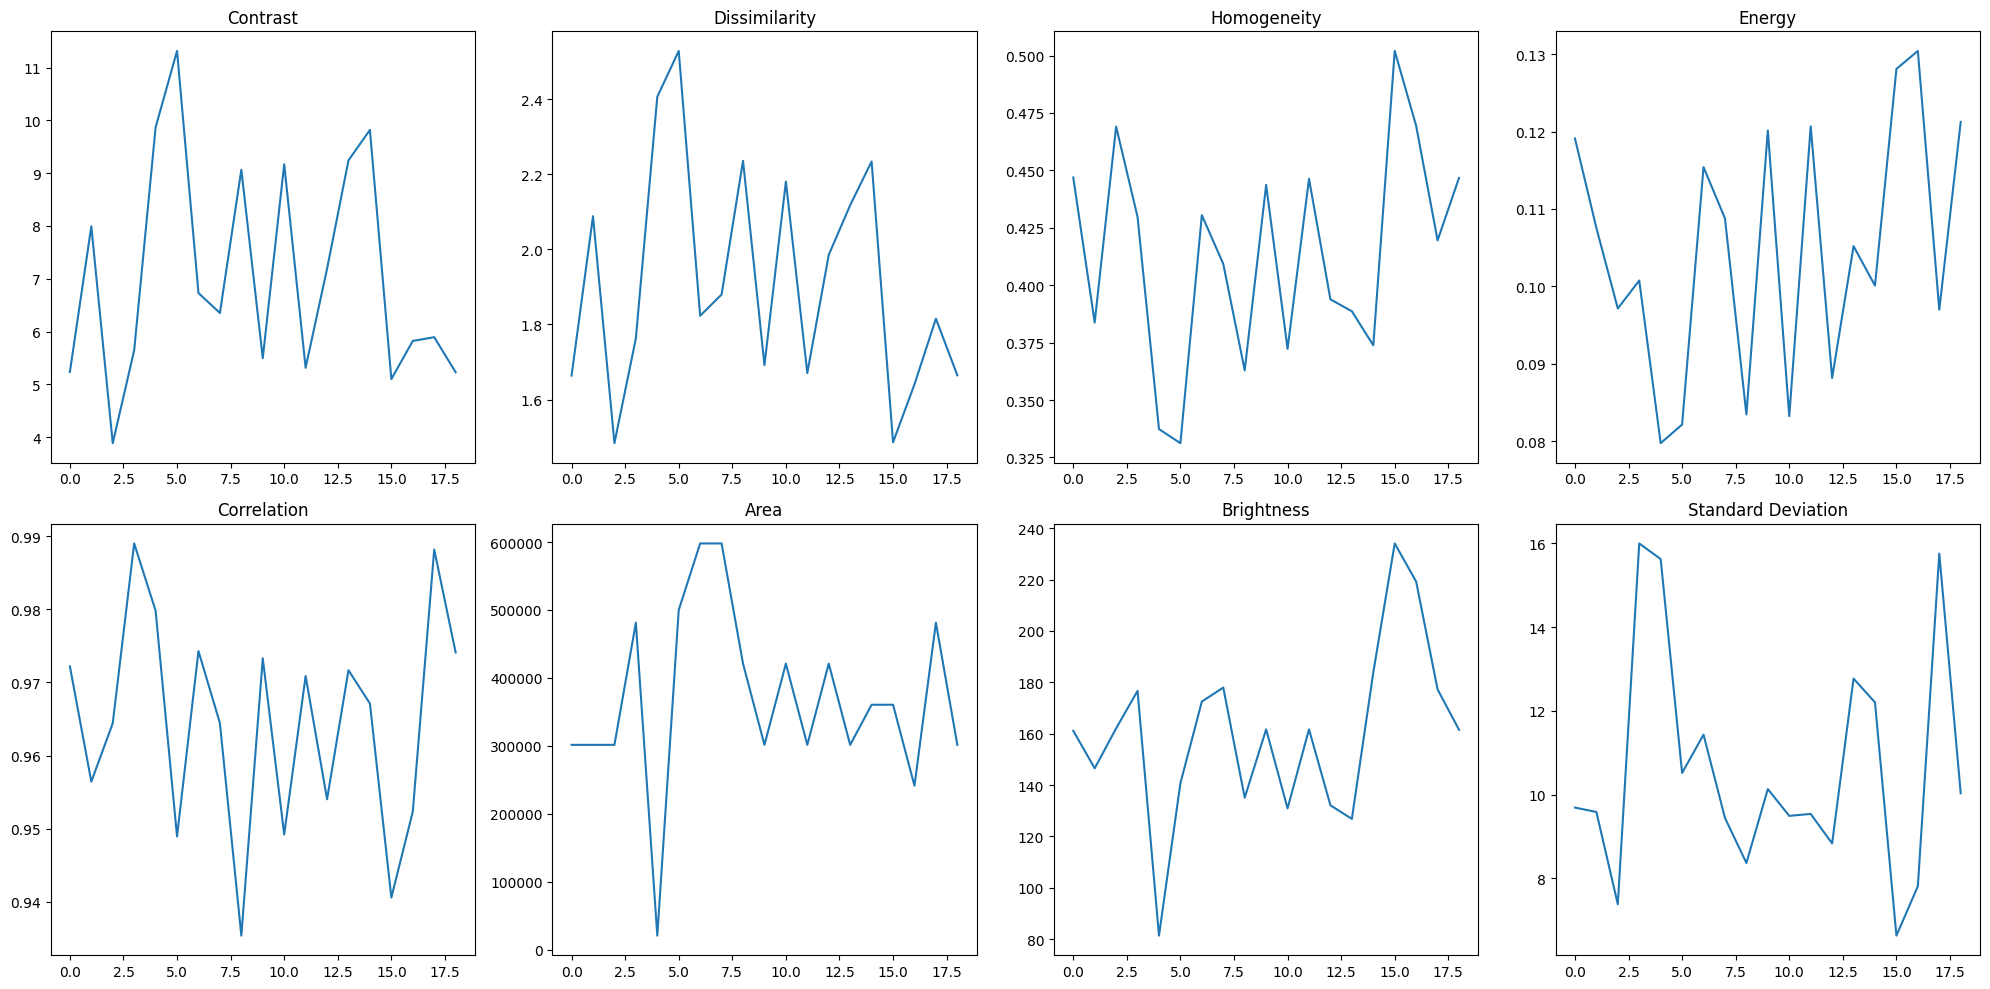
\includegraphics[width=\textwidth]{Figures/EDA_Charts/9/da.png}
        \caption*{Data Analysis}
    \end{minipage}
    \caption{Image Folder G Analysis}
    \label{fig:Image Folder G Analysis}
\end{figure}

\subsection{Image Folder H}

There are 14 JPEG files totalling a size of 6.16mb in Image Folder H. The images are of varying dimensions.

\begin{figure}[ht]
    \centering
    \begin{minipage}[t]{0.25\textwidth}
        \centering
        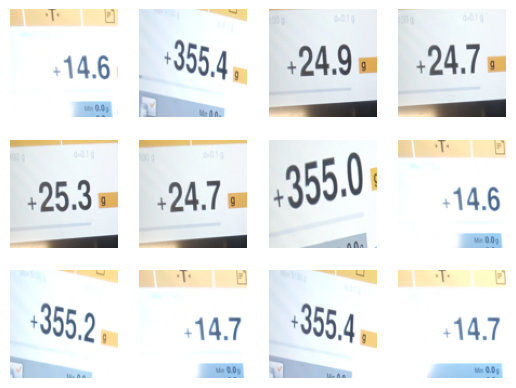
\includegraphics[width=\textwidth]{Figures/EDA_Charts/11/montage.png}
        \caption*{Montage}
    \end{minipage}\hfill
    \begin{minipage}[t]{0.25\textwidth}
        \centering
        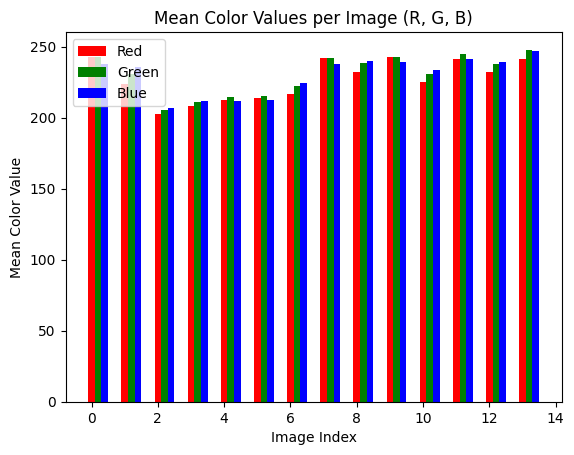
\includegraphics[width=\textwidth]{Figures/EDA_Charts/11/rgb.png}
        \caption*{RGB}
    \end{minipage}\hfill
    \begin{minipage}[t]{0.50\textwidth}
        \centering
        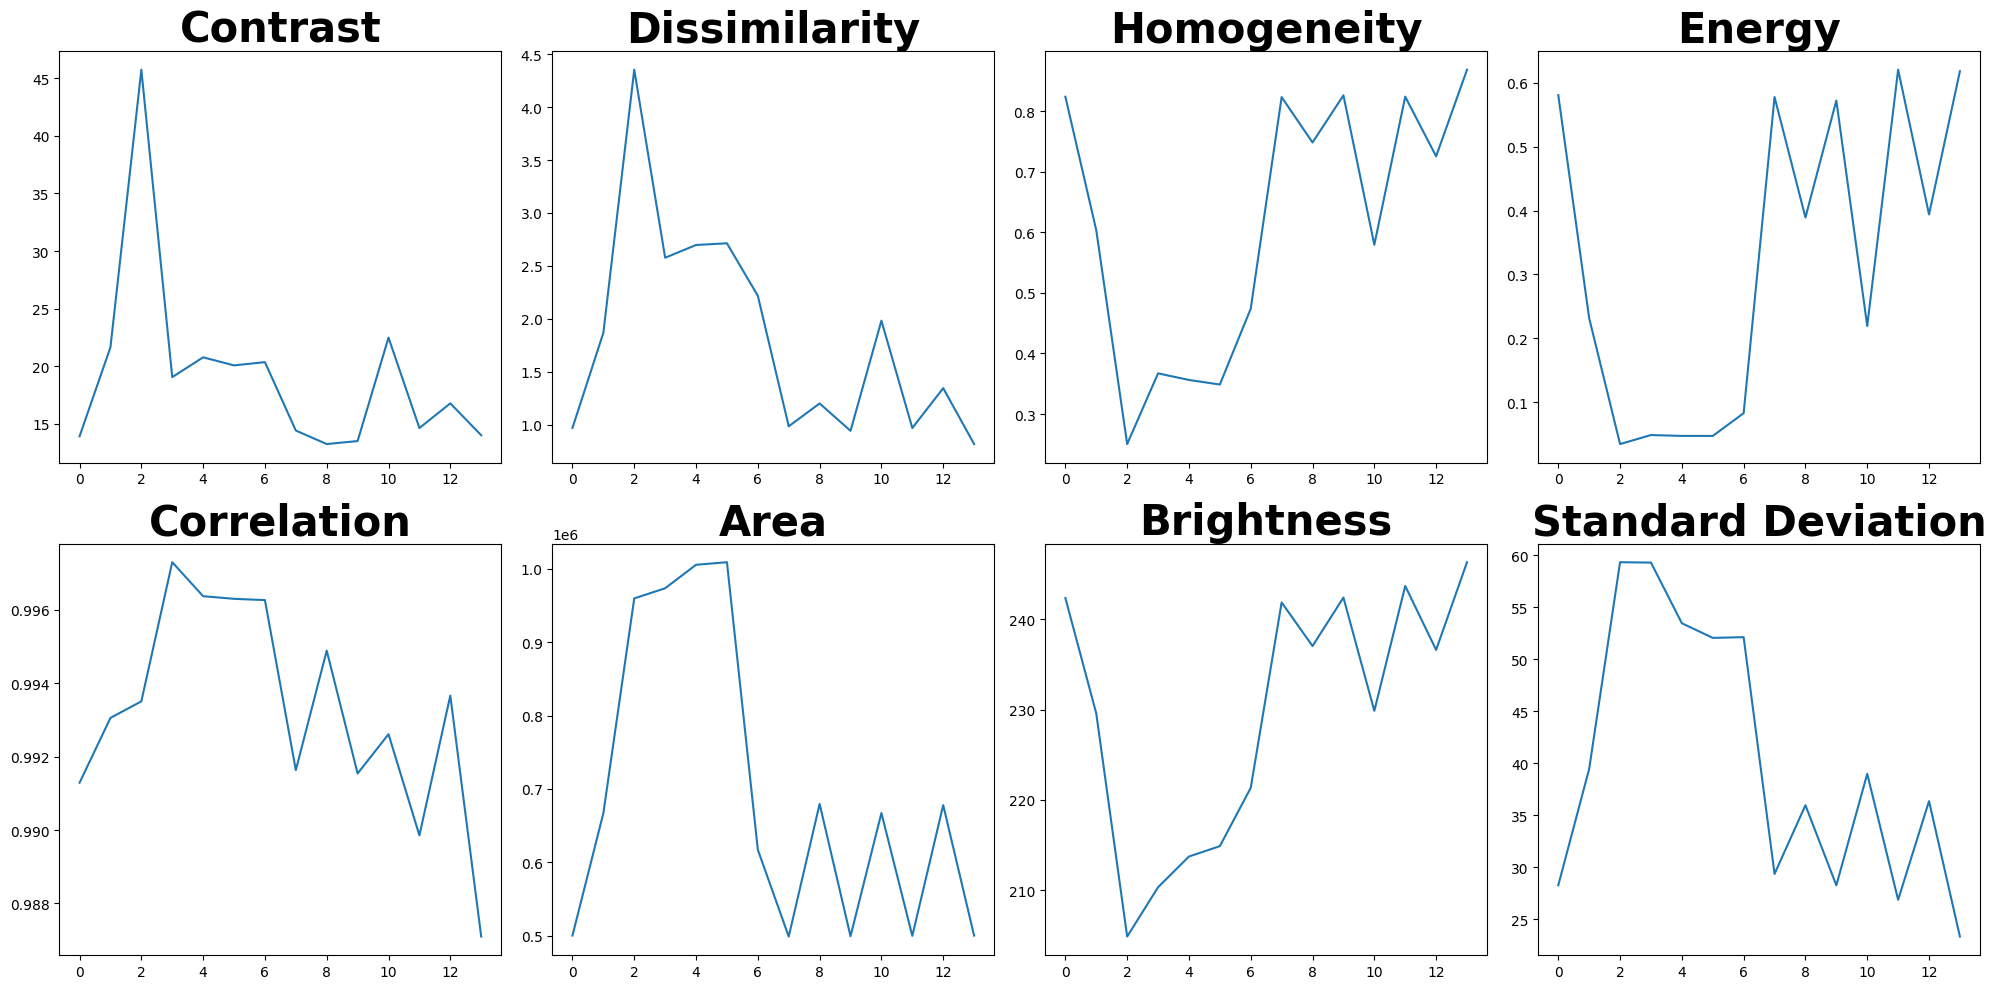
\includegraphics[width=\textwidth]{Figures/EDA_Charts/11/da.png}
        \caption*{Data Analysis}
    \end{minipage}
    \caption{Image Folder H Analysis}
    \label{fig:Image Folder H Analysis}
\end{figure}


\newpage

\section{First Sprint - Global Generic}


\textbf{Objective:} To successfully perform Optical Character Recognition (OCR) on the entire dataset of images using the pytesseract library, while implementing and evaluating the impact of image pre-processing techniques, specifically the conversion of images to greyscale, to optimize OCR accuracy.

Utilizing the pytesseract library's Python interface for the Tesseract OCR engine, this sprint delves into the practical execution of our objective, focusing on the nuances of image pre-processing.

\begin{figure}[ht]
    \centering
    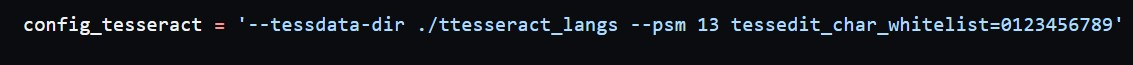
\includegraphics[width=0.9\textwidth]{Figures/firstrun/tesseract_config.jpg}
    \caption[PyTesseract Config Settings]{PyTesseract Config Settings}
    \label{fig:PyTesseract Config Settings}
\end{figure}


The pre-processing here involves turning the image to greyscale. Converting a colour image to greyscale is a process of condensing the three colour channels (Red, Green, and Blue) into a single channel that represents the image's brightness. This is done by applying specific weights to each channel, which mimic the way the human eye perceives colour. The weights used are 0.2989 for red, 0.5870 for green, and 0.1140 for blue. This process reduces the amount of data required to represent the image, which can simplify many image processing tasks. \cite{cadikPerceptualEvaluationColortoGrayscale2008}

\begin{figure}[h]
    \centering
    \begin{minipage}{0.45\textwidth}
        \centering
        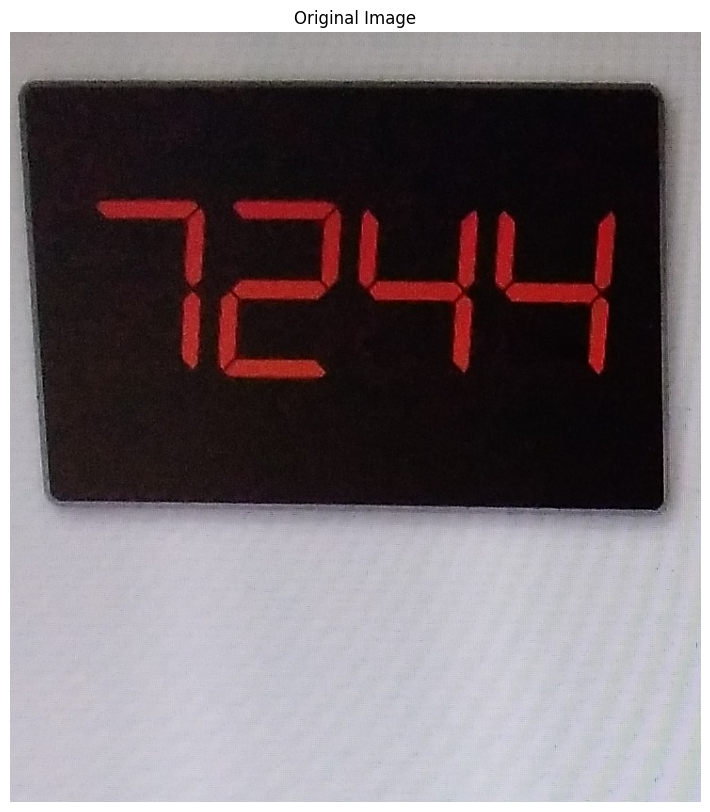
\includegraphics[width=0.9\textwidth]{Figures/gray/original.png}
        \caption*{Original Image}
    \end{minipage}\hfill
    \begin{minipage}{0.45\textwidth}
        \centering
        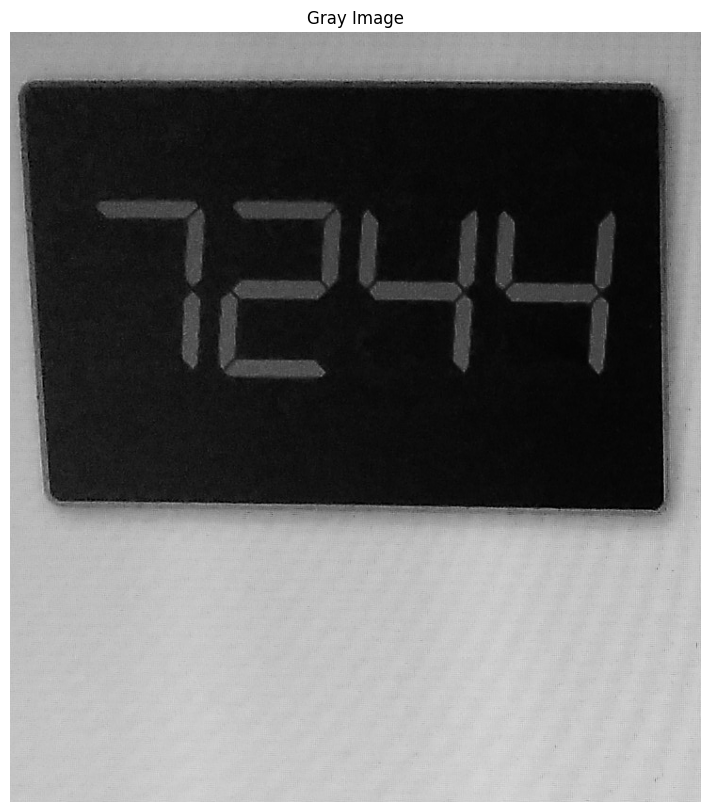
\includegraphics[width=0.9\textwidth]{Figures/gray/grey.png}
        \caption*{Greyscale Image}
    \end{minipage}
    \caption{Greyscale Conversion}
\end{figure}

\subsection{Conclusion for the First Sprint}
In this sprint, we successfully implemented OCR on our dataset using the pytesseract library. The greyscale conversion pre-processing technique was crucial in optimizing the accuracy of the OCR. The specific configurations, as depicted in Fig 3.11, were adjusted to maximize results, with settings of PSM 6, 7, and particularly 13, yielding the most accurate readings. Detailed insights and implications of these findings will be further elaborated in the main Results and Conclusion chapters.

\newpage

\section{Second Sprint - Global Generic Analysis Resized}

\textbf{Objective for the Second Sprint:}
To enhance the accuracy of OCR results from the initial sprint by integrating advanced pre-processing techniques, including Otsu's thresholding, morphological closing, and image resizing. Furthermore, the sprint aims to utilize specialized Tesseract language files, adapting OCR to specific textual representations, thereby ensuring a more tailored and precise text recognition process across diverse image sets.

Building upon the foundation established in the first sprint, the second sprint introduced several pivotal enhancements. Otsu's thresholding and morphological closing were integrated into the pre-processing pipeline. Additionally, a novel resizing technique was employed alongside the inclusion of a seven-segment display language file, collectively augmenting the OCR system's accuracy. Each of these advancements deepens our exploration into the realm of OCR optimization.

\subsection*{Method - Otsu's Thresholding}

Otsu's method is a global thresholding technique used in image processing. It is named after its inventor, Nobuyuki Otsu, and works by minimizing the intraclass variance, which is a measure of how similar the pixels within each class are. The optimal threshold value is the one that produces the two classes with the lowest intraclass variance. \cite{garciaDetectionClassificationPathogens2021}

\begin{figure}[h]
    \centering
    \begin{minipage}{0.45\textwidth}
        \centering
        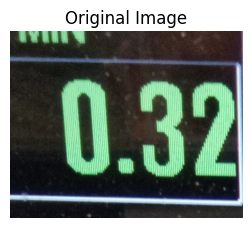
\includegraphics[width=0.9\textwidth]{Figures/otsu/original.png}
        \caption*{Original Image}
    \end{minipage}\hfill
    \begin{minipage}{0.45\textwidth}
        \centering
        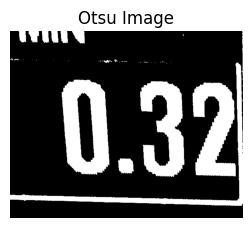
\includegraphics[width=0.9\textwidth]{Figures/otsu/otsu.png}
        \caption*{Otsu's Thresholding}
    \end{minipage}
    \caption{Otsu's Thresholding}
\end{figure}

Once the optimal threshold value has been determined, the image can be binarized, which means converting it to a black and white image. In this sprint, the pixels with values below the threshold will be set to black, and the pixels with values above the threshold will be set to white.

\subsection*{Method - Morphological Closing}

Morphological closing is an image processing operation that is used to close small holes in the foreground of an image. In OpenCV, closing is performed by first applying a dilation operation, which grows or thickens objects in the image, followed by an erosion operation, which shrinks objects in the image. The size and shape of the area affected by each operation depends on the structuring element used. The overall effect of the closing operation is that small holes within an object, thin lines or gaps between objects, and small black points on the object are eliminated, while keeping the size and shape of the object roughly the same as before the operation. This operation is particularly useful in many image processing tasks, such as noise reduction and separation of touching objects. \cite{haralickImageAnalysisUsing1987}

\begin{figure}[h]
    \centering
    \begin{minipage}{0.30\textwidth}
        \centering
        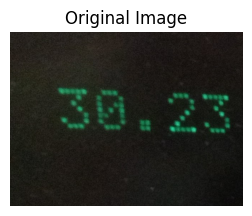
\includegraphics[width=0.9\textwidth]{Figures/closing/original.png}
        \caption*{Original}
    \end{minipage}\hfill
    \begin{minipage}{0.30\textwidth}
        \centering
        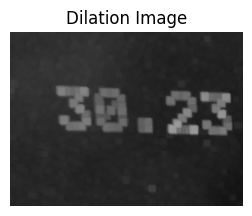
\includegraphics[width=0.9\textwidth]{Figures/closing/dilated.png}
        \caption*{Dilated}
    \end{minipage}\hfill
    \begin{minipage}{0.30\textwidth}
        \centering
        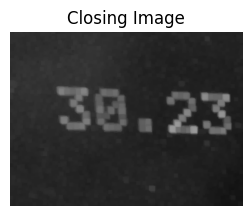
\includegraphics[width=0.9\textwidth]{Figures/closing/closing.png}
        \caption*{Closing}
    \end{minipage}
    \caption{Morphological Closing}
\end{figure}

\subsection*{Method - Tesseract Language Files}

The lang parameter that can be passed into Tesseract specifies the language of the text to be recognized. Tesseract is capable of recognizing text in multiple languages. To utilize this functionality, the appropriate language data files must be downloaded and installed. These files can be found on the Tesseract GitHub page. \cite{Tessdata2023}

\begin{figure}[ht]
    \centering
    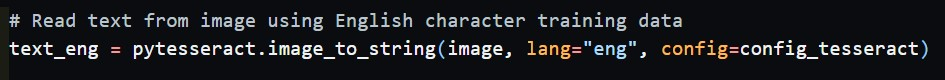
\includegraphics[width=0.9\textwidth]{Figures/second_run/lang.jpg}
    \caption[PyTesseract Config Settings Language]{PyTesseract Config Settings Language}
    \label{fig:PyTesseract Config Settings - Language}
\end{figure}


The language files used in this research are as follows:

\begin{itemize}
    \item eng.traineddata - English
    \item ssd.traineddata - Seven Segment Display
\end{itemize}


\subsection*{Method - Resizing}

To improve the results of optical character recognition (OCR) using Tesseract, image resizing during pre-processing was explored. Tesseract's performance can be sensitive to the scale of the image, as the size of the text can greatly impact the OCR engine's ability to accurately recognize characters. Therefore, resizing images to various scales became an essential part of the pre-processing pipeline.

Resizing is performed using OpenCV's resize() function, which allows images to be scaled up or down. By altering the resolution, the text in the images is effectively manipulated to appear larger or smaller. It is worth noting that while upscaling can sometimes help in capturing more detail and thereby improving OCR accuracy, it also increases computational load. Conversely, downscaling an image reduces the computational burden but might cause loss of important details that can negatively affect OCR performance. \cite{dasCovid19FaceMask2020}


The Python script was redesigned to run the control function in a loop incrementally adjusting the image resize parameter from 50 pixels to 749 pixels and evaluating the subsequent influence on Optical Character Recognition (OCR) performance. The aim was to find an ideal image size that would not make the text too small or too large, thus optimizing the recognition potential of Tesseract.


\subsection{Second Sprint Conclusion}

Conducting OCR on diverse image sets presents challenges due to their wide-ranging attributes, including differences in colour profiles, lighting conditions, text styles, and noise levels. Such variability underscores a key insight: a one-size-fits-all pre-processing pipeline for Tesseract may not be adequate. Embracing a more adaptive and tailored strategy is essential.

The power of OpenCV, an expansive open-source computer vision library, is harnessed in this sprint to provide granular image processing capabilities. By tailoring pre-processing steps for each specific image folder—whether it's grayscale conversion, Gaussian blurring, adaptive thresholding, or even morphological transformations—we're able to cater to the unique needs of each dataset. This meticulous adjustment, although intricate, was pivotal in enhancing OCR accuracy.

The process highlighted not just the intricacies of fine-tuning OCR techniques but also illuminated a key takeaway: the essence of flexibility. Global strategies, while appealing in their broad applicability, may not always produce the desired outcomes. It's often the detailed, customized methods that yield superior results, especially when dealing with diverse datasets.

\newpage

\section{Third Sprint - Analysis Tesseract Separate Folders}

\textbf{Objective for the Third Sprint:} To further refine the Optical Character Recognition (OCR) capabilities across a variety of image sets by introducing specialized pre-processing techniques tailored to each folder's distinct properties. Techniques such as Red Mask, Green Mask, Deblurring, Thresholding, and Skewness Correction were employed. Additionally, the sprint aimed to address specific challenges presented by each image set, such as diverse colour profiles, skewness, and noise, ensuring the highest possible OCR accuracy.

The diverse attributes of the images in the dataset, ranging from colour profiles to skewness, posed intricate challenges for OCR using Tesseract. Instead of applying a one-size-fits-all approach, this sprint underscored the importance of adaptability. In the ensuing sections, we delve deeper into advanced pre-processing techniques, notably highlighting the Red Mask application via OpenCV. The focus remains on customizing processes for individual image subsets, showcasing the project's commitment to precision and tailored solutions.


\subsection*{Method - Red Mask}

The Red Mask function operates on an input image to isolate and return only the red pixels in that image.

The input image should be a numpy ndarray representing the original image in BGR format. To process this, the function first converts the image into the HSV (Hue, Saturation, Value) colour space using OpenCV's cvtColor function.

\begin{figure}[h]
    \centering
    \begin{minipage}{0.45\textwidth}
        \centering
        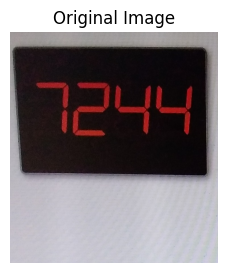
\includegraphics[width=0.9\textwidth]{Figures/red_mask/original.png}
        \caption*{Original Image}
    \end{minipage}\hfill
    \begin{minipage}{0.45\textwidth}
        \centering
        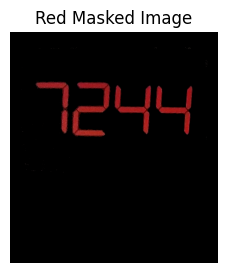
\includegraphics[width=0.9\textwidth]{Figures/red_mask/red_mask.png}
        \caption*{Red Mask Image}
    \end{minipage}
    \caption{Red Mask}
\end{figure}


Because the hue component of red colour in HSV space spans both ends of the hue spectrum, two ranges are defined to capture the entire red hue — the lower range (0-10) and the higher range (170-180). These ranges are combined with saturation and value thresholds to define what is considered a red pixel in the image.

The function then creates two binary masks for these ranges, using OpenCV's inRange function, which applies these boundaries on the HSV image. The resulting masks have pixel values of 255 where the original image pixels are within the specified red range, and 0 otherwise.

\begin{figure}[ht]
    \centering
    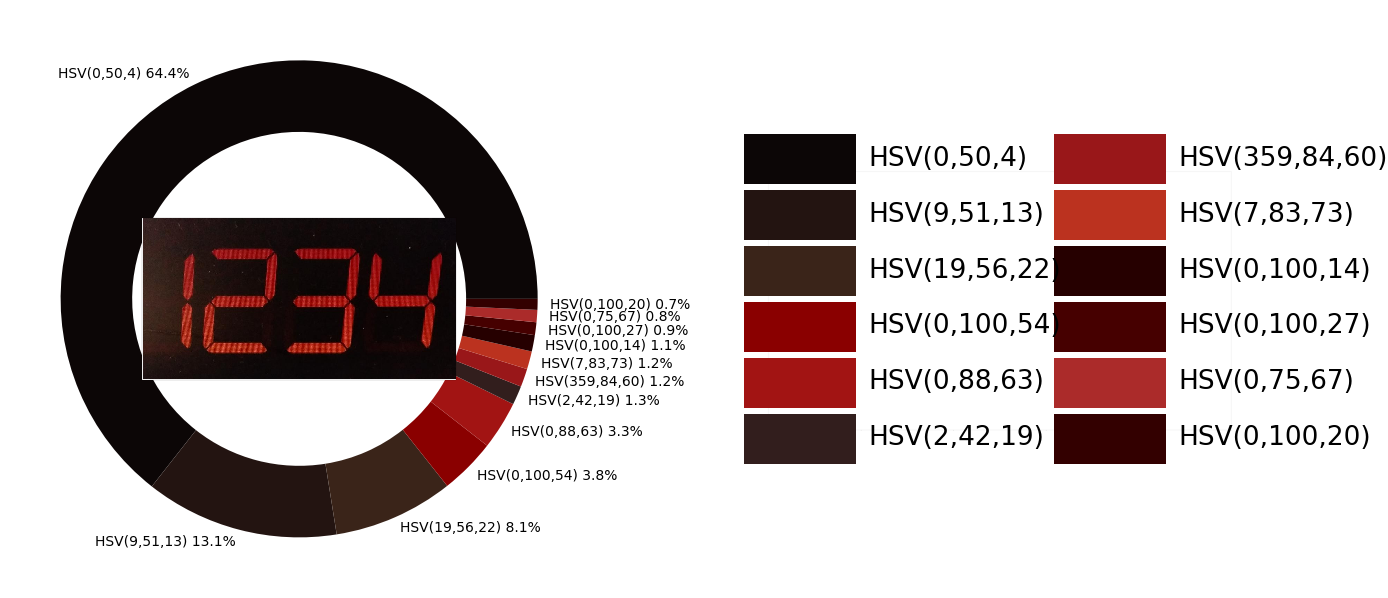
\includegraphics[width=0.9\textwidth]{Figures/Methodology/sipa_02/red_analysis.png}
    \caption[Colour Analysis]{Colour Analysis}
    \label{fig:Colour Analysis}
\end{figure}


These two masks are added together to form a comprehensive mask of red pixels. The function then applies this mask onto a copy of the original image, setting all the pixels where the mask equals 0 to also be 0 in the output image. This leaves only the red pixels visible in the output image. Hence, the function returns an image emphasizing the red components of the original input.


\newpage

\subsection{Image Folder A}

\begin{figure}[ht]
    \centering
    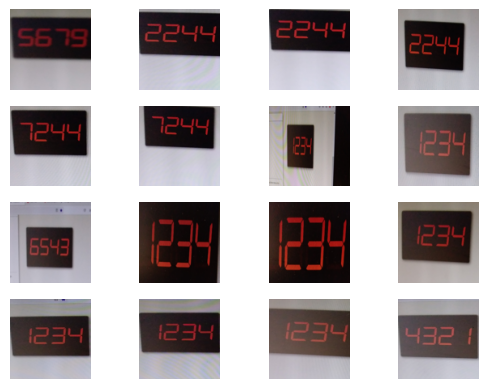
\includegraphics[width=0.9\textwidth]{Figures/EDA_Charts/2/montage.png}
    \caption[Image Folder A Montage]{Image Folder A Montage}
    \label{fig:Image Folder A Montage}
\end{figure}

The methodology for processing images in Folder A involved the following steps:

\begin{enumerate}
    \item An initial exploratory analysis was conducted where the images were resized to sizes ranging from 50 to 649 pixels in both height and width. This was done to empirically determine the optimal size that yields the best results in subsequent processing and text extraction steps.
    \item After analysing the results, an image size of 104 pixels was found to be the optimal size and was used for further processing of the images.
    \item A Red Mask was applied. The significance and process of this technique has been previously explained in the Introduction.
    \item The images were then converted to grayscale to reduce computational complexity and focus on intensity values.
    \item The OTSU method was applied to further process the images. The choice of this method is discussed in the Introduction.
    \item Text was extracted using the ENG and SSD Tesseract training libraries, which were chosen for their proven efficiency and accuracy in optical character recognition tasks.
    \item The process was repeated with the additional step of using morphological operations of Closing and Dilation, in order to remove noise and enhance the accuracy of text extraction.
    \item The results from each step and the final output were saved to a CSV file for further analysis and interpretation.
\end{enumerate}

\begin{figure}[ht]
    \centering
    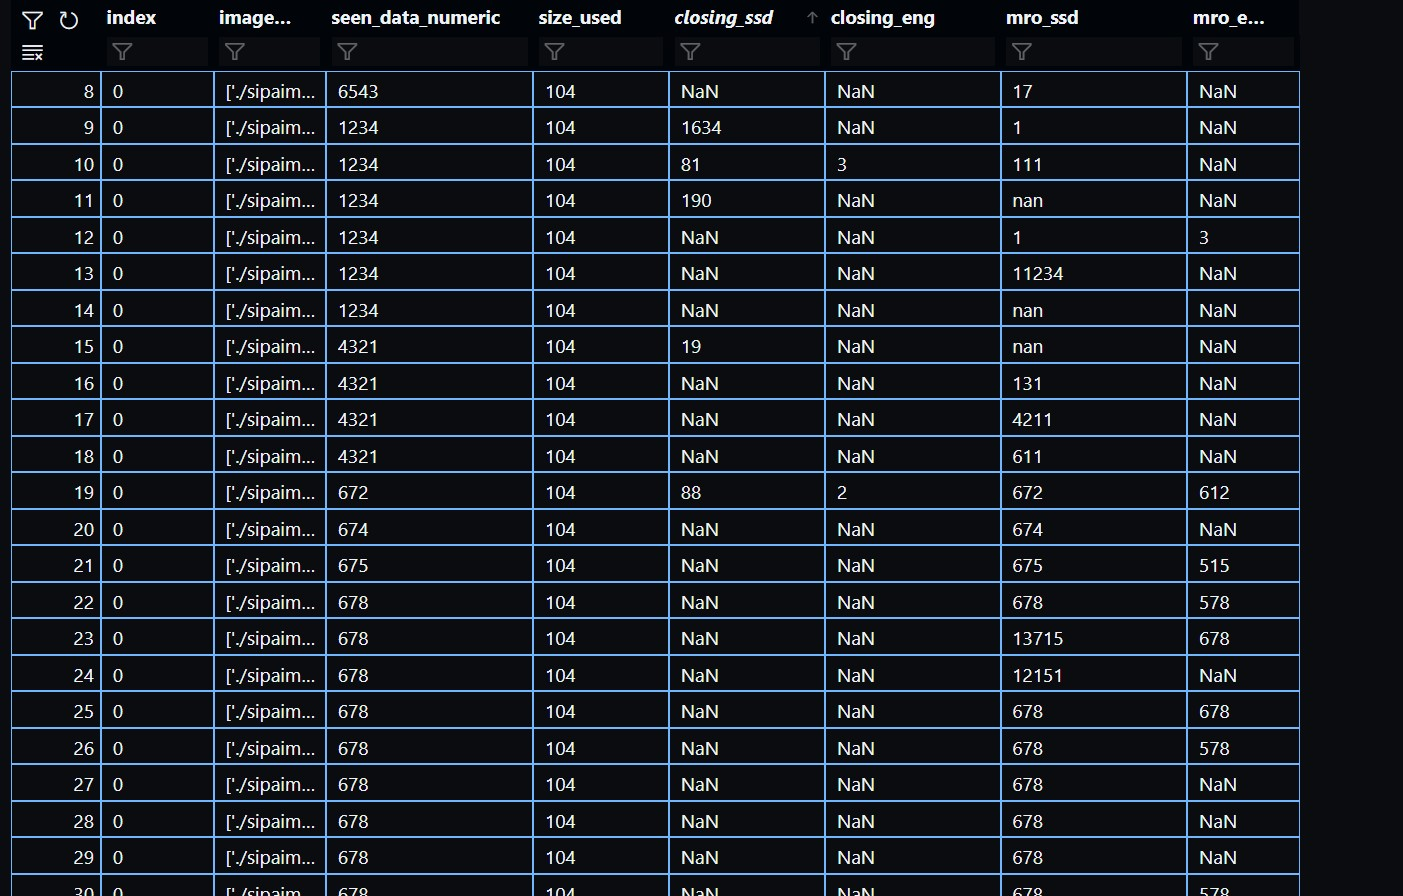
\includegraphics[width=0.9\textwidth]{Figures/Methodology/sipa_02/sample_output.jpg}
    \caption[Image Folder A Sample Output]{Image Folder A Sample Output}
    \label{fig:Image Folder A Sample Output}
\end{figure}

The figure above presents a sample of the output generated from the Image Folder A analysis. This analysis file is discussed in the Results section of this document.

\newpage
\subsection{Image Folder B}

\begin{figure}[ht]
    \centering
    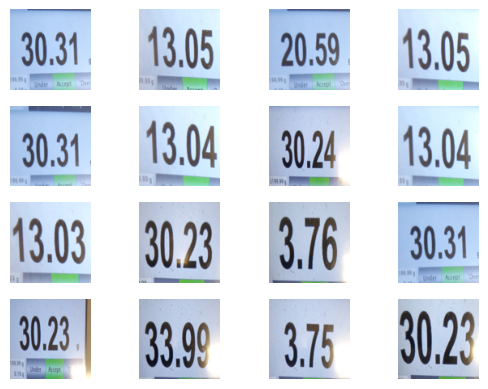
\includegraphics[width=0.9\textwidth]{Figures/EDA_Charts/3/montage.png}
    \caption[Image Folder B Montage]{Image Folder B Montage}
    \label{fig:Image Folder B Montage}
\end{figure}

The methodology for processing images in Folders A and B involved the following steps:

\begin{enumerate}
    \item An initial exploratory analysis was conducted where the images were resized to sizes ranging from 50 to 649 pixels in both height and width. This was done to empirically determine the optimal size that yields the best results in subsequent processing and text extraction steps.
    \item After analysing the results, an image size of 550 pixels was found to be the optimal size and was used for further processing of the images.
    \item An initial pre-processing function of thresholding (thresh) was applied. This method helps in separating an object from its background and improves the overall contrast of the images.
    \item Following the thresholding step, the images underwent morphological closing operations. This technique, which involves dilation followed by erosion, is used to close small holes in the object, making the images cleaner for further processing.
    \item The OTSU method was applied as a final pre-processing step to binarize the images. This adaptive thresholding method maximizes inter-class variance and improves the precision of text extraction, as discussed in the Introduction.
    \item Text was extracted using the ENG and SSD Tesseract training libraries, chosen for their proven efficiency and accuracy in optical character recognition tasks.
    \item The results from each pre-processing step and the final output were saved to a CSV file for further analysis and interpretation.

\end{enumerate}

\begin{figure}[ht]
    \centering
    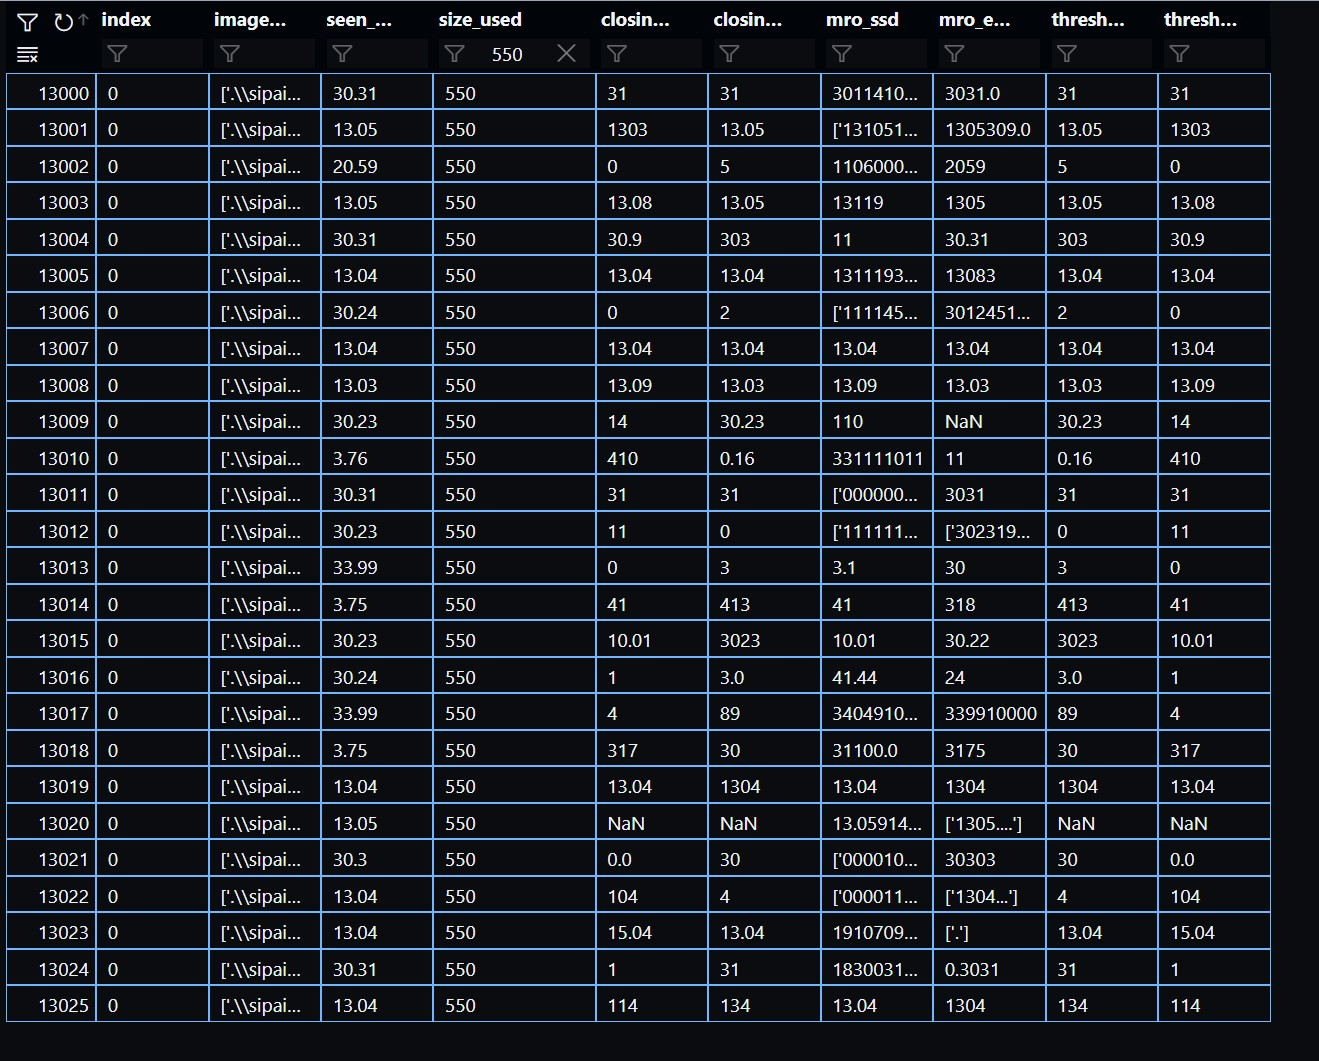
\includegraphics[width=0.9\textwidth]{Figures/Methodology/sipa_03/sample_output.jpg}
    \caption[Image Folder B Sample Output]{Image Folder B Sample Output}
    \label{fig:Image Folder B Sample Output}
\end{figure}

\newpage

\subsection{Image Folder C}

Two new methods were introduced for working with Image Folder C.

\subsection*{Method - Denoise}

The \textit{cv2.fastNlMeansDenoisingColored} function in OpenCV is a fast algorithm for denoising colour images. It works by converting the image to CIELAB colour space and then denoising the L and AB components separately. The denoising is done using a non-local means algorithm, which works by finding similar patches in the image and averaging them together. The parameters of the algorithm can be adjusted to control the amount of denoising. \cite{OpenCVDenoising}

The \textit{cv2.fastNlMeansDenoisingColoured} function takes the following parameters:


\begin{itemize}
    \item \textbf{src}: The input image.
    \item \textbf{dst}: The output image.
    \item \textbf{h}: The parameter that controls the amount of denoising for the L component.
    \item \textbf{hColour}: The parameter that controls the amount of denoising for the AB components.
    \item \textbf{templateWindowSize}: The size of the template patch used for denoising.
    \item \textbf{searchWindowSize}: The size of the search window used for denoising.
\end{itemize}

The \texttt{cv2.fastNlMeansDenoisingColoured} function is a fast and effective way to denoise colour images. It is particularly well-suited for images that have been corrupted by Gaussian noise.\cite{OpenCVDenoising}

\subsubsection*{Method - Weiner Filter}

The Wiener filter is a linear filter that is used to denoise signals that have been corrupted by additive white Gaussian noise (AWGN). The Wiener filter is optimal in the sense that it minimizes the mean-squared error between the denoised signal and the original signal.

The Wiener filter is defined as follows:

\begin{figure}[htbp]
    \centering
    \begin{equation}
        w(f) = K \cdot R_xx^{-1} \cdot R_xn
    \end{equation}
    \caption{Weiner Filter Equation} \cite{priyadarshiniComparativePerformanceAnalysis2022}
\end{figure}

The Wiener filter can mitigate the effects of sunlight, treated as additive white Gaussian noise, on an image. It estimates the sunlight's power spectrum, applying its inverse to the image, thus reducing sunlight while preserving the original signal. The Wiener filter can be implemented through:

\begin{itemize}
    \item Frequency domain: Adjusting the image using the inverse of the sunlight's power spectrum.
    \item Time domain: Utilizing a recursive algorithm.
\end{itemize}

However, it may produce ringing artifacts and requires precise knowledge of the sunlight's power spectrum for effective results.


\begin{figure}[ht]
    \centering
    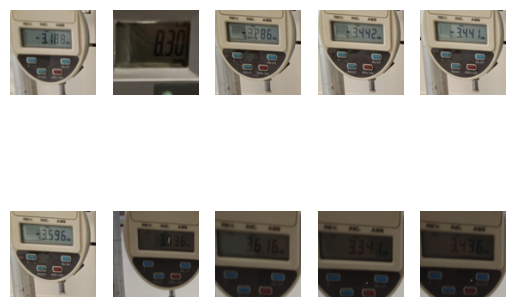
\includegraphics[width=0.9\textwidth]{Figures/EDA_Charts/4/montage.png}
    \caption[Image Folder C Montage]{Image Folder C Montage}
    \label{fig:Image Folder C Montage}
\end{figure}

The methodology for Image Folder C was developed to maximize the readability and accuracy of the extracted text from the images. The following steps were taken:

\begin{figure}[ht]
    \centering
    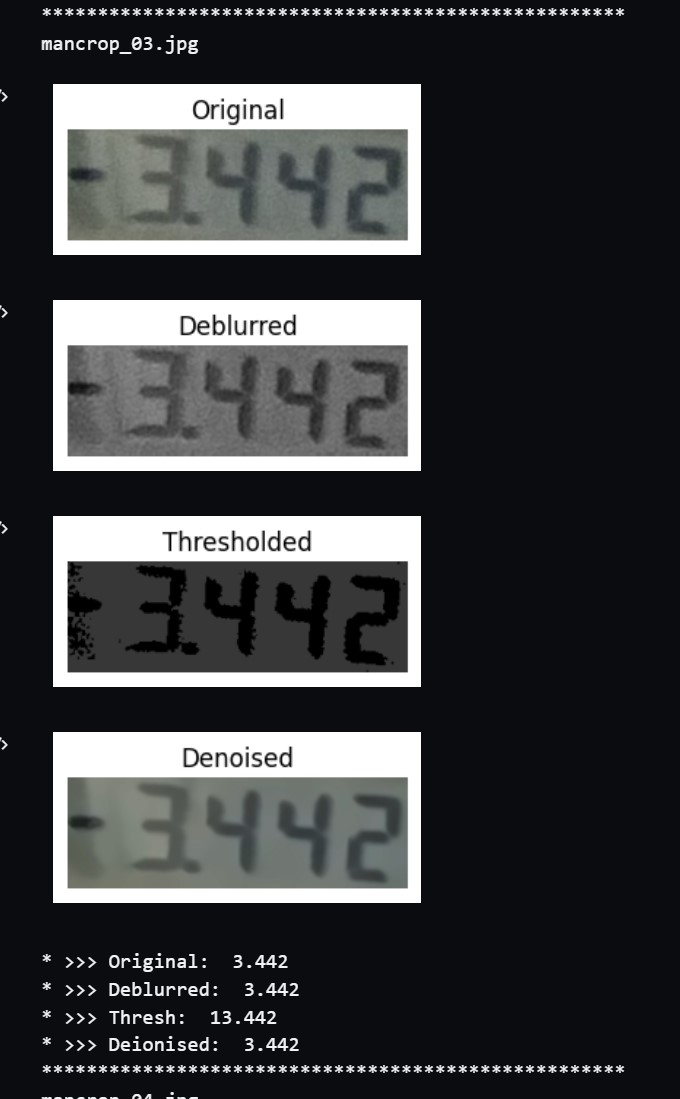
\includegraphics[width=0.4\textwidth]{Figures/Methodology/sipa_04/result_sample.jpg}
    \caption[Image Folder C Sample Output]{Image Folder C Sample Output}
    \label{fig:Image Folder C Sample Output}
\end{figure}


\begin{enumerate}
    \item \textbf{Manual Cropping}: Images were manually cropped to isolate the text. This process was necessary to ensure that only the relevant portions of the images were analysed. It is important to note that this manual step could be avoided with more precise camera positioning during the initial image capture phase.
    \item \textbf{Deblurring}: A deblurring operation was performed on the images using the Wiener filter. This step was necessary to reduce the blur caused by linear motion or unfocused optics.
    \item \textbf{Thresholding}: The images underwent a thresholding operation. This process was required to help separate the text (foreground) from the background, improving the contrast and readability of the text.
    \item \textbf{Denoising}: The images were denoised to reduce the noise present. This step was essential to further enhance the clarity and readability of the text.
    \item \textbf{Text Extraction and Accuracy Assessment}: Text was extracted from the processed images. To evaluate the accuracy of the extraction, the extracted text was compared with predefined labels. The text that matched the predefined label the closest was considered to be the most accurate.
\end{enumerate}

\newpage

\subsection{Image Folder D}


\begin{figure}[ht]
    \centering
    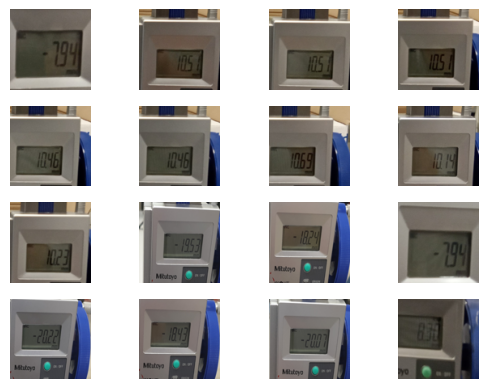
\includegraphics[width=0.9\textwidth]{Figures/EDA_Charts/5/montage.png}
    \caption[Image Folder D Montage]{Image Folder D Montage}
    \label{fig:Image Folder D Montage}
\end{figure}

The methodology for Image Folder D involved a series of systematic steps to accurately read the text within the images and output the analysis to a CSV file. The procedure followed is detailed below:

\begin{enumerate}
    \item \textbf{Image Cropping:} The text within the images was manually cropped. While this method was chosen for its simplicity and effectiveness, the necessity of this step could be mitigated in the future by improving the camera positioning to automatically focus on the text.

    \item \textbf{Grayscale Conversion:} The cropped images were then converted to grayscale. This step is crucial as it simplifies the image, reduces computational complexity, and is preferred for most image processing tasks such as the OCR (Optical Character Recognition) used in this project.

    \item \textbf{Median Blurring:} The grayscale images underwent a median blur process. This step helps in reducing noise within the images, thereby enhancing the efficiency of the OCR.

    \item \textbf{Text Recognition:} The processed images were then used to read text using Optical Character Recognition (OCR) with English language (ENG) and Seven Segment Display (SSD) configuration files. The SSD configuration, an algorithm for object detection, aids in accurately identifying and locating the text within the image.

    \item \textbf{Data Export:} Finally, the text recognized from the images was analysed, and the output was exported to a CSV file for further analysis and record-keeping.
\end{enumerate}

\begin{figure}[ht]
    \centering
    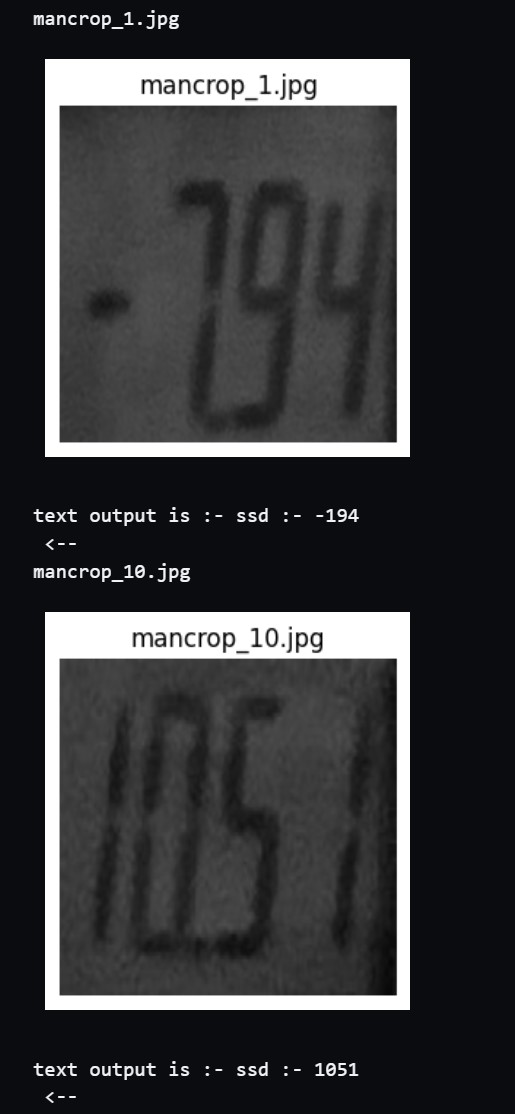
\includegraphics[width=0.3\textwidth]{Figures/Methodology/sipa_05/sample_output.jpg}
    \caption[Image Folder D Sample Output]{Image Folder D Sample Output}
    \label{fig:Image Folder D Sample Output}
\end{figure}

\newpage

\subsection{Image Folder E}

\begin{figure}[ht]
    \centering
    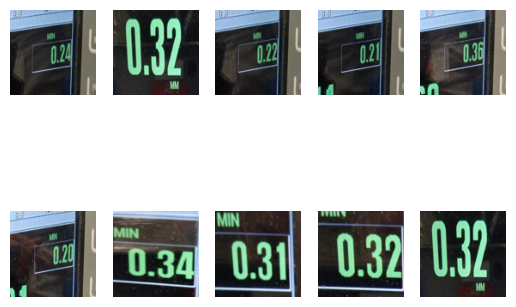
\includegraphics[width=0.9\textwidth]{Figures/EDA_Charts/7/montage.png}
    \caption[Image Folder E Montage]{Image Folder E Montage}
    \label{fig:Image Folder E Montage}
\end{figure}

In this section, a function similar to the previously discussed Red Mask technique is introduced and utilized. This new function, termed the 'Green Mask', operates under similar principles but targets green pixel values instead of red.

\subsection*{Method - Green Mask}

The Green Mask function isolates and returns only the green pixels in an input image. The input image is a numpy ndarray representing the original image in BGR format. The function first converts the image into the HSV (Hue, Saturation, Value) colour space using OpenCV's cvtu function.

In the HSV colour space, green occupies a certain section of the hue spectrum. A specific range is defined to capture the green hue, typically around 36-70. This range, along with specific thresholds for saturation and value, defines what is considered a green pixel in the image.

\begin{figure}[h]
    \centering
    \begin{minipage}{0.45\textwidth}
        \centering
        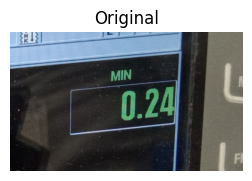
\includegraphics[width=0.9\textwidth]{Figures/green_mask/original.png}
        \caption*{Original Image}
    \end{minipage}\hfill
    \begin{minipage}{0.45\textwidth}
        \centering
        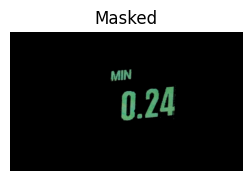
\includegraphics[width=0.9\textwidth]{Figures/green_mask/green_mask.png}
        \caption*{Green Mask Image}
    \end{minipage}
    \caption{Green Mask}
\end{figure}


The function then creates a binary mask for this range using OpenCV's inRange function. This function applies the boundaries of the defined range to the HSV image, resulting in a mask with pixel values of 255 where the original image pixels are within the specified green range, and 0 otherwise.

The function then applies this mask onto a copy of the original image, setting all the pixels where the mask equals 0 to also be 0 in the output image. This leaves only the green pixels visible in the output image. Therefore, the function returns an image emphasizing the green components of the original input.

The methodology for Image Folder E utilized a sequential process to efficiently read text within the images and subsequently output the analysis to a CSV file. The steps involved in the process are as follows:

\begin{enumerate}
    \item \textbf{Image Cropping:} The text within the images was manually cropped. This task, while manually intensive, could be avoided in future iterations by optimizing camera positioning to directly focus on the text.

    \item \textbf{Green Mask Application:} A green mask was applied to the images to isolate specific features or areas of interest in the image, enhancing the subsequent image processing steps.

    \item \textbf{Grayscale Conversion:} The masked images were then converted to grayscale. This step reduces computational complexity and is a standard pre-processing step in many image processing workflows, including OCR (Optical Character Recognition).

    \item \textbf{Deblurring:} A deblurring operation was performed on the grayscale images to enhance the clarity and legibility of the text in the images.

    \item \textbf{Thresholding:} Thresholding was applied to the deblurred images, converting them into a binary format. This step helps in separating the text (foreground) from the background.

    \item \textbf{Denoising:} The binary images underwent a denoising process to further reduce noise and improve the effectiveness of the subsequent OCR process.

    \item \textbf{Text Recognition:} The denoised images were then used to read text using Optical Character Recognition (OCR) with English language (ENG) and Seven Segment Display (SSD) configuration files. SSD configuration, a method for object detection, is used to accurately identify and locate the text within the images.

    \item \textbf{Data Export:} The recognized text from the images was analysed, and the output was exported to a CSV file for further analysis and record-keeping.
\end{enumerate}

Every step was conducted with precision to ensure the accuracy of the results and the effectiveness of the method employed.

\begin{figure}[ht]
    \centering
    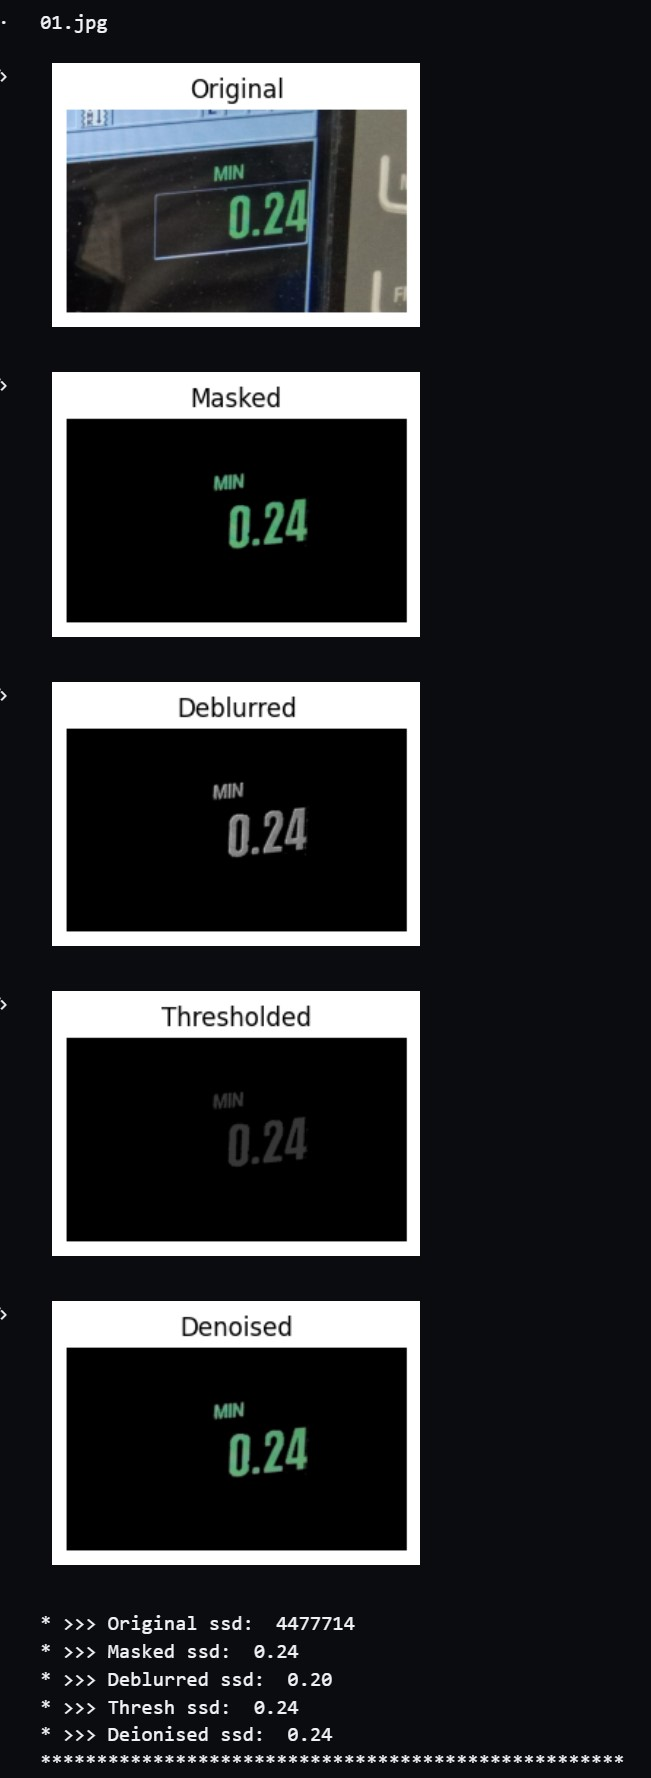
\includegraphics[width=0.2\textwidth]{Figures/Methodology/sipa_07/sample_output.jpg}
    \caption[Image Folder E Sample Output]{Image Folder E Sample Output}
    \label{fig:Image Folder E Sample Output}
\end{figure}


\newpage

\subsection{Image Folder F}

\begin{figure}[ht]
    \centering
    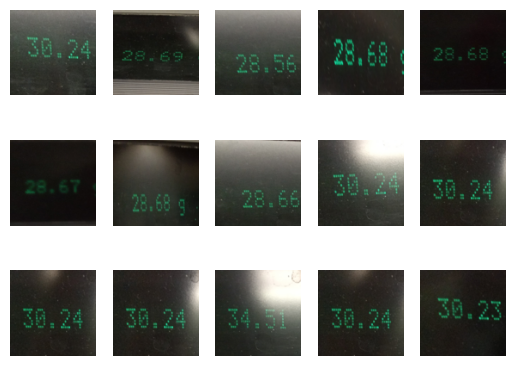
\includegraphics[width=0.9\textwidth]{Figures/EDA_Charts/8/montage.png}
    \caption[Image Folder F Montage]{Image Folder F Montage}
    \label{fig:Image Folder F Montage}
\end{figure}

The methodology for Image Folder F utilized a sequential process to efficiently read text within the images and subsequently output the analysis to a PDF file. The steps involved in the process are as follows:


\begin{enumerate}
    \item \textbf{Image Cropping:} The text within the images was manually cropped. This task, while manually intensive, could be avoided in future iterations by optimizing camera positioning to directly focus on the text.
    \item \textbf{Mask Green}: Apply a green colour mask to images. This step isolates the green parts of the image for further processing.
    \item \textbf{Grayscale}: Convert the masked image to grayscale. This step simplifies the image and is a common requirement for many image processing algorithms.
    \item \textbf{Deblur}: Deblur the grayscale image. This step sharpens the image, enhancing details for the OCR.
    \item \textbf{Threshold}: Apply a thresholding technique on the deblurred image. This step separates the image into foreground and background, aiding in the recognition of text.
    \item \textbf{OCR}: Use Tesseract OCR on the processed images. This step recognizes text in various languages and fonts, including English (ENG), SSD, and Dot Matrix.
    \item \textbf{PDF Generation}: Use the ReportLab library in Python to create a PDF of the OCR results. This step provides a convenient way to view and share the results.
\end{enumerate}

\begin{figure}[ht]
    \centering
    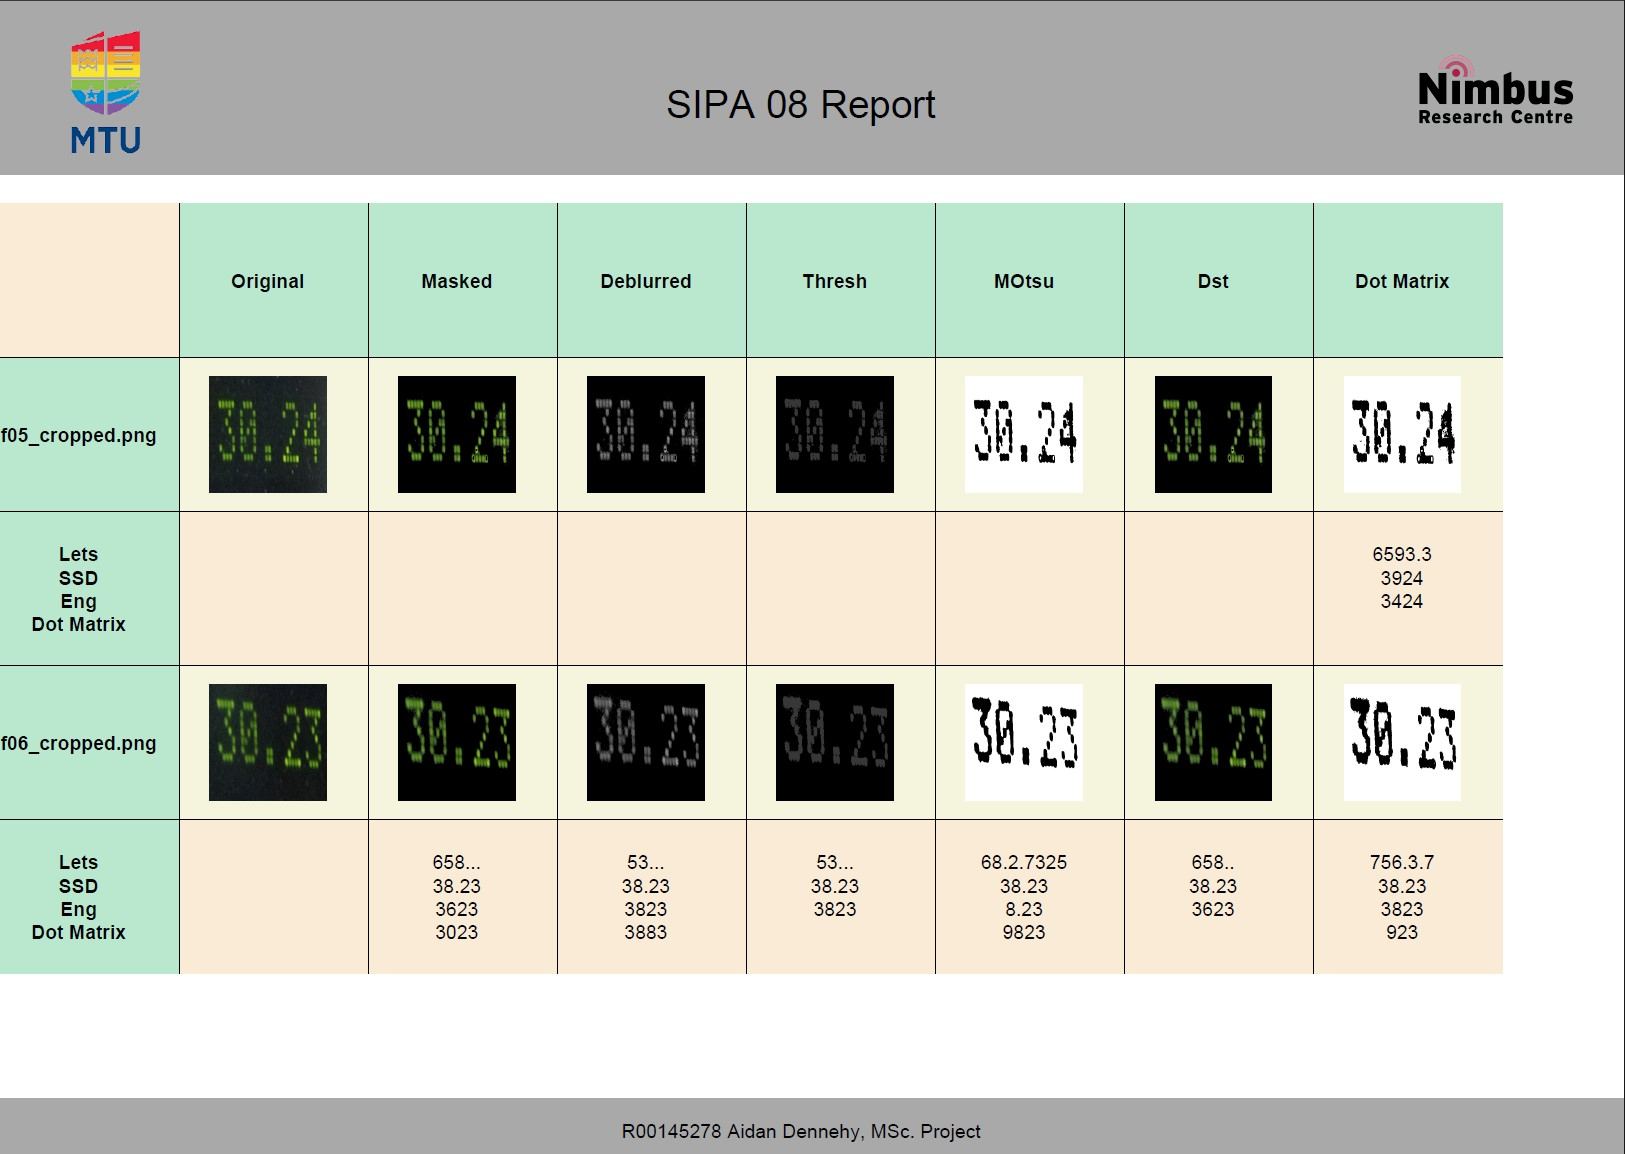
\includegraphics[width=0.8\textwidth]{Figures/Methodology/sipa_08/sample_output.jpg}
    \caption[Image Folder F Sample Output]{Image Folder F Sample Output}
    \label{fig:Image Folder F Sample Output}
\end{figure}


\newpage

\subsection{Image Folder G}

\begin{figure}[ht]
    \centering
    \includegraphics[width=0.9\textwidth]{Figures/EDA_Charts/9/montage.png}
    \caption[Image Folder G Montage]{Image Folder G Montage}
    \label{fig:Image Folder G Montage}
\end{figure}

The methodology for Image Folder G used a sequential process to read text within the images efficiently and output the analysis to a PDF file. The steps involved in the process were as follows:

\begin{enumerate}
    \item \textbf{Manual Crop}: Manually crop the image to focus on the area of interest and remove any irrelevant parts.
    \item \textbf{Convert to Grayscale}: Convert the cropped image to grayscale. This simplifies the image, reducing the amount of information to process, and is a common requirement for many image processing algorithms.
    \item \textbf{Invert Image}: Invert the grayscale image. This step switches the light and dark areas of the image, which can sometimes help in improving OCR results.
    \item \textbf{Threshold Grayscale Image}: Apply a thresholding technique to the inverted grayscale image. This step separates the image into foreground and background, aiding in the recognition of text.
    \item \textbf{OCR Using Tesseract}: Use Tesseract OCR on the threshold image. Run Tesseract with multiple configurations, using the SSD, LetsGoDigital, DotMatrix, and ENG language models, to find the best result.
    \item \textbf{PDF Generation}: Use the ReportLab library in Python to create a PDF of the OCR results. This step provides a convenient way to view and share the results.
\end{enumerate}

\begin{figure}[ht]
    \centering
    \includegraphics[width=0.8\textwidth]{Figures/Methodology/sipa_09/sample_output.jpg}
    \caption[Image Folder G Sample Output]{Image Folder G Sample Output}
    \label{fig:Image Folder G Sample Output}
\end{figure}

\newpage
\subsection{Image Folder H}

\begin{figure}[ht]
    \centering
    \includegraphics[width=0.9\textwidth]{Figures/EDA_Charts/11/montage.png}
    \caption[Image Folder H Montage]{Image Folder H Montage}
    \label{fig:Image Folder H Montage}
\end{figure}

Black text on a white background is a good scenario for OCR. The main problem with these images above is skewness.

A function was developed to estimates the rotation angle of an image by detecting lines using the Hough Transform. \cite{mukhopadhyaySurveyHoughTransform2015} The function first converts the image to grayscale and applies the Canny edge detector to find edges. It then uses the Hough Transform to detect lines in the image. If no lines are detected, it returns 0. Otherwise, it calculates the angles of the detected lines, and computes and returns the median of these angles as the estimated rotation angle.

The methodology for processing images in Folder H involved the following steps:

\begin{enumerate}
    \item \textbf{Manual Crop}: Manually crop the image to focus on the area of interest and remove any irrelevant parts.
    \item \textbf{Correct Skewness}: Correct the skewness of the image using the Hough Transform.
    \item \textbf{OCR Using Tesseract}: Use Tesseract OCR on the corrected image using the ENG model.

\end{enumerate}

\begin{figure}[ht]
    \centering
    \includegraphics[width=0.6\textwidth]{Figures/Methodology/sipa_11/sample_output.jpg}
    \caption[Image Folder H Sample Output]{Image Folder H Sample Output}
    \label{fig:Image Folder H Sample Output}
\end{figure}


\subsection{Third Sprint Conclusion}

In the Third Sprint, the project delved deeper into the nuances of OCR by catering to specific challenges presented by each image set. Addressing the multifaceted nature of the images, individualized pre-processing techniques were employed for each folder. From leveraging colour masks like the Red and Green Masks to correct skewness using the Hough Transform, the methodologies were designed for optimized results. Notably, the sprint showcased the importance of adaptability and specificity, affirming that while global strategies offer a foundational approach, it's the fine-tuned, tailored interventions that ensure precision and excellence. The outcome of this sprint was a testament to the project's evolving capabilities, highlighting that with each iteration, the OCR process becomes increasingly robust and reliable.

\newpage

\section{Fourth Sprint - CRNN Methodology}

\textbf{Objective for the Fourth Sprint:} To harness the combined strengths of Convolutional Neural Networks (CNNs) and Recurrent Neural Networks (RNNs) by implementing and fine-tuning a Convolutional Recurrent Neural Network (CRNN) methodology for Optical Character Recognition (OCR). The sprint encompasses the creation of a bespoke digit dataset tailored to specific image fonts, model architecture definition, data preparation and pre-processing, culminating in accurate digit predictions. The overarching goal is to achieve superior OCR accuracy by capitalizing on the spatial and sequential processing capabilities of the CRNN.

\subsection{Introduction}

In this subsection, the specifics of utilizing Convolutional Recurrent Neural Networks (CRNNs) for the task are discussed. The CRNN, a hybrid model, harnesses the spatial feature extraction capabilities of CNNs with the sequence modelling prowess of RNNs. The subsequent sections guide through the systematic process: from building the training databases to defining the architecture of the CRNN model, followed by data preparation through loading, normalization, and one-hot encoding. Finally, the model's compilation and the prediction of numbers are addressed.


\subsection{Building the Training Databases}
While initial experiments with the CRNN utilized the MNIST \cite{MnistTensorFlowDatasets} and SVHN \cite{StreetViewHouse} datasets for training, results indicated that a custom digits training database, tailored to the specific font present in the images, yielded the most optimal performance.

In this research, a Python-based approach was employed to generate random images of individual digits using a specified font. The Python Imaging Library (PIL) was used to perform image manipulations. The process begins by determining the desired font.

\begin{figure}[ht]
    \centering
    \includegraphics[width=0.4\textwidth]{Figures/find_font/myfonts.jpg}
    \caption[Image Font Identification]{Image Font Identification}
    \label{fig:Image Font Identification}
\end{figure}

The process involved using font identification websites such as \textit{www.myfonts.com}\cite{WhatTheFontMyFonts}, but generally the best success was attained by looking for similar fonts on Google Fonts \cite{BrowseFontsGoogle}. The font was then downloaded and installed on the local machine.

The primary function is tasked with producing a designated number of digit images and saving them in a predetermined directory. Each digit image file is labelled with a randomly generated alphanumeric name, followed by an underscore and the digit it represents.

To enhance the diversity of the dataset, digits are rendered in varying font sizes. Additionally, there's a 50\% chance that any given image will undergo a slight rotation within a specified range. This introduces a semblance of natural variability that might be found in real-world digit representations, mimicking minor skews or rotations.

After the image creation, all the generated image file names, along with their respective digits, are documented in a structured format. This record, which acts as a catalogue, is then appended to a designated CSV file. The CSV provides a ready reference, allowing researchers to quickly correlate an image file to its corresponding digit without visual interpretation.

This methodology ensures a vast and varied dataset, essential for robust machine learning training or any analysis requiring a diverse representation of numerical digits.


\subsection{Defining the CRNN Model}

To instantiate the model in our experiment, we set the \texttt{input\_shape} to be (32, 32, 1), as our pre-processed images are 32x32 pixels with 1 channel (grayscale). The number of output classes, \texttt{num\_classes}, is set to 10 to represent the digits from 0 to 9.

\begin{verbatim}
input_shape = (32, 32, 1)
num_classes = 10
crnn_model = create_crnn_model(input_shape, num_classes)
\end{verbatim}

The structure of the instantiated model is as follows:

\begin{itemize}
    \item \textbf{Input Layer}: The model takes an input of shape \texttt{input\_shape} (32, 32, 1) in our case.
    \item \textbf{Convolutional Layers}: The first part of our model comprises three convolutional blocks. Each block consists of:
          \begin{itemize}
              \item \textbf{Convolutional Layer}: Uses a varying number of filters, starting from 32, then 64, and finally 128, all with a kernel size of 3x3 and 'same' padding.
              \item \textbf{Batch Normalization}: Normalizes the outputs of the convolutional layers.
              \item \textbf{ReLU Activation}: Introduces non-linearity, enabling the model to learn complex patterns.
              \item \textbf{Max Pooling}: Reduces the spatial dimensions of the output.
              \item \textbf{Dropout}: Applied with a rate of 0.25 to prevent overfitting.
          \end{itemize}
    \item \textbf{Reshaping Layer}: The output of the convolutional layers is reshaped to a target shape of (4, 4*128) for the LSTM layer.
    \item \textbf{Recurrent Layers}: A Bidirectional LSTM layer with 256 units processes the reshaped sequences, followed by a TimeDistributed Dense layer with ReLU activation.
    \item \textbf{Flattening and Dropout}: The output from the TimeDistributed layer is flattened and passed through a Dropout layer with a rate of 0.5.
    \item \textbf{Output Layer}: A Dense layer with \texttt{num\_classes} units (10 in our case) and a softmax activation function classifies the images. This layer also uses L1 and L2 regularization.
\end{itemize}

This model structure is chosen because it capitalizes on the strengths of both Convolutional Neural Networks (CNNs) and Recurrent Neural Networks (RNNs). Specifically, the CNN layers are adept at processing spatial information and extracting important features from the input images, making them ideal for image recognition tasks. Following this, the sequential patterns in these extracted features are processed by an RNN layer (specifically an LSTM), which is proficient in learning from temporal or sequential data. This combination, often referred to as a Convolutional Recurrent Neural Network (CRNN), can be particularly effective in tasks like digit recognition, where recognizing both spatial features (e.g., shape of the digits) and sequential dependencies (e.g., order of strokes in handwritten digits) can be beneficial.

\subsection{Loading the Training Data}
In the methodology, the dataset generated of 500k seven segment digits is loaded. Each image corresponds to a specific digit that is labelled in a corresponding csv file. A load function is utilized to read and process these images. The images are accessed with their respective file names, read into memory as grayscale images using the OpenCV library.

Following this, each image is resized to a uniform size of 32x32 pixels, ensuring that the input to our model remains consistent. The images are then expanded along the last axis to create an additional dimension, a standard pre-processing step required by the Convolutional Neural Networks (CNNs). This dimension effectively represents the colour channels of the image, which in our case is one, due to the use of grayscale images. The processed images are then stored in a list, which is converted into a numpy array for efficient numerical operations.


To validate the model's performance and generalization capabilities, the dataset is divided into a training and  testing set, using an 80-20 split. This split is achieved by using the \textit{train\_test\_split} function from the Scikit-learn library. The resulting subsets are X\_train and y\_train for the training set, and X\_test and y\_test for the testing set, where 'X' represents the images and 'y' the corresponding labels. The \textit{random\_state} parameter is arbitrarily fixed at 42, providing reproducibility in the generation of the training and testing splits. This approach facilitates the reservation of a significant portion of the dataset for model training while ensuring a distinct set remains for evaluating the model's ability to generalize to unseen data.

\subsection{Normalisation and One-Hot Encoding}
The datasets are normalised and one-hot encoded to facilitate the training process. Normalisation is achieved by dividing the pixel values by the maximum grayscale value, which is 255. This transformation reduces the scale of input values, facilitating the convergence of our model during the training process. One-hot encoding is performed using the \textit{to\_categorical} function from the TensorFlow Keras utility module. This function converts the training and test labels (y\_train and y\_test) into one-hot vectors, a format required by the model algorithms when dealing with categorical targets. Each digit from 0-9 is represented as a 10-element vector with a single '1' in the position representing the digit and '0's elsewhere.

\subsection{Model Compilation}
The model is compiled using the \textit{compile} function from the TensorFlow Keras API. The model employs the Adam optimization algorithm, a popular choice due to its efficient memory usage and capability to handle large datasets and parameters. The \textit{categorical\_crossentropy} is set as the loss function, which is suitable for multi-class classification tasks. The 'accuracy' of model is tracked as a metric during the training process.

The batch size, set at 64, defines the number of samples that will be passed through the network at one time. This number represents a balance between computational efficiency and the stochastic nature of the learning process. The number of epochs, set at 25, represents the number of times the entire training dataset will be passed forward and backward through the neural network.

The training process starts with the fit function. Here, X\_train and y\_train are the training images and labels respectively. The training proceeds with a batch size of 64 and for 25 epochs as defined earlier. The model's performance is evaluated on the validation dataset, X\_test and y\_test, after each epoch, providing a view on the model's ability to generalize from the training data to unseen data. The output from this function, including the loss and accuracy of the model after each epoch, is saved to the history variable for potential later analysis.

\subsection{Image Folder Pre-processing}

Several functions were developed to cater to the unique characteristics of the image folder and its segmentation requirements. These functions transform the image to grayscale, streamlining the process for subsequent contour detection. Contours falling below a certain area threshold are filtered out, ensuring only meaningful segments are retained. The accepted contours are organized based on their x-coordinates, which guarantees a sequential extraction of digits. For each pertinent contour, a bounding box is drawn, and segments meeting the area criteria are isolated as individual digits. The collective output of these functions comprises both the valid contours and the segmented digits, equipping the system for any further analysis or operations.

\subsection{Prediction of Numbers}

Each segmented is resized to the target size, the pixel values are normalized to the range [0, 1], and dimensions adjusted to be compatible the CRNN model input expectations, specifically by adding channel and batch axes.

After pre-processing the binary digit image, the model predicts its value, and the digit's identity is determined by selecting the index with the highest prediction score.

\begin{figure}[ht]
    \centering
    \includegraphics[width=0.4\textwidth]{Figures/Results/crnn/sample_predict.jpg}
    \caption[Image Prediction via CRNN]{Image Prediction via CRNN}
    \label{fig:Image Prediction via CRNN}
\end{figure}

\newpage

\subsection{Fourth Sprint Conclusion}

Throughout the fourth sprint, the focus has been the integration and fine-tuning of Convolutional Recurrent Neural Network (CRNN) methodologies for Optical Character Recognition (OCR). This hybrid model, which synergizes the spatial prowess of CNNs with the sequential expertise of RNNs, was found to be significantly adept at recognizing digits, especially when trained on custom datasets tailored to specific fonts in the images.

Our comprehensive exploration began with generating an expansive and varied training dataset. Emphasis was placed on the quality and diversity of the dataset, ensuring the CRNN model was exposed to an array of digit representations, mimicking real-world nuances. The meticulous process of defining the CRNN model architecture was undertaken, capitalizing on the complementary strengths of CNNs and RNNs. This was followed by data preparation steps, involving loading, normalization, and one-hot encoding to ensure data compatibility with the model.

The segment on Image Folder Pre-processing underlined the importance of accurate segmentation. The methods employed not only ensured efficient digit extraction but also catered to the unique characteristics of each image set. The sprint culminated in the prediction phase, where the trained CRNN model was leveraged to discern digit identities with high accuracy.

In essence, this sprint has showcased the efficacy of CRNNs in the realm of OCR, demonstrating its potential in handling both spatial and sequential intricacies inherent in the task. The detailed breakdown, from data generation to prediction, serves as a testament to the rigorous approach adopted in this phase, solidifying the foundation for subsequent sprints and investigations.

% \subsection{Conclusion}

% In this chapter, an exploration of the research methodology has been presented. The primary objective being the enhancement of the performance of Optical Character Recognition (OCR) systems, with a specific focus on Tesseract OCR and Convolutional Recurrent Neural Network (CRNN) models. A systematic approach was employed, initiating a global run of OCR systems on raw image datasets. This highlighted the pivotal role of image pre-processing in augmenting OCR results. The importance of pre-processing, especially the application of colour masks before grayscale conversion, was underscored as a method to improve image clarity and subsequently the efficiency of the OCR processes. Serving as a detailed roadmap, the chapter elucidated each phase of the research methodology, from the initial evaluation of OCR systems to the intricate details of the pre-processing techniques.

\section{Methodology Chapter Conclusion}

This chapter details the research methodology, emphasizing dedicated efforts to enhance the performance of Optical Character Recognition (OCR) systems. Specifically, the focus on Tesseract OCR and the Convolutional Recurrent Neural Network (CRNN) models led to a comprehensive evaluation of OCR systems using unprocessed image datasets.

Data capture, as outlined in Objective 2, equipped the study with a diverse set of sensor reading images, reflecting the multifaceted nature of the subject under investigation.

Objective 3 guided the exploration of image pre-processing techniques, prominently featuring colour masking before grayscale conversion. This method aimed to sharpen image clarity, setting the stage for better OCR results.

In alignment with Objective 4, the research delved into pinpointing optimal image capture settings. This exploration, combined with pre-processing, framed a strategy to enhance OCR precision and efficiency.

In essence, this chapter stands as a thorough guide, mapping out the methodology and addressing the initial four objectives of the research. It spans from initial OCR system assessments to the details of refined pre-processing methods and the nuances of optimal image capture settings.



